% ============================================================================
%  Reference Validity and Symmetry-Sector Consistency in Quantum-Chemical
%  Benchmarks
%
%  Compile:  pdflatex main.tex     (run twice: ToC + cross-references)
%  No bibtex pass required -- the bibliography is inline.
%  Figures expected in ./figures/
% ============================================================================
\documentclass[11pt,a4paper]{article}

\usepackage[T1]{fontenc}
\usepackage[utf8]{inputenc}
\usepackage{lmodern}
\usepackage[margin=2.4cm,headheight=14pt]{geometry}
\usepackage{amsmath,amssymb}
\usepackage{graphicx}
\usepackage{booktabs}
\usepackage{array}
\usepackage{caption}
\usepackage{enumitem}
\usepackage{fancyhdr}
\usepackage{microtype}
\usepackage{xcolor}

\definecolor{NavyLink}{HTML}{1A4C8B}
\definecolor{BoxBlue}{HTML}{EAF1F9}
\definecolor{BoxRule}{HTML}{1A4C8B}
\definecolor{WarnBg}{HTML}{FDF3E7}
\definecolor{WarnRule}{HTML}{9C5B12}
\definecolor{StopBg}{HTML}{F5EEEE}
\definecolor{StopRule}{HTML}{8B1A1A}

\usepackage{tcolorbox}
\usepackage[colorlinks=true,linkcolor=NavyLink,citecolor=NavyLink,
            urlcolor=NavyLink,bookmarksnumbered=true]{hyperref}

% ---------------------------------------------------------------- callouts --
\newtcolorbox{result}[1][]{%
  colback=BoxBlue, colframe=BoxRule, boxrule=0.7pt, arc=1.5pt,
  left=6pt, right=6pt, top=5pt, bottom=5pt,
  fonttitle=\bfseries\sffamily\small, title={#1}}

\newtcolorbox{caution}[1][]{%
  colback=WarnBg, colframe=WarnRule, boxrule=0.7pt, arc=1.5pt,
  left=6pt, right=6pt, top=5pt, bottom=5pt,
  fonttitle=\bfseries\sffamily\small, title={#1}}

\newtcolorbox{unsupported}[1][]{%
  colback=StopBg, colframe=StopRule, boxrule=0.7pt, arc=1.5pt,
  left=6pt, right=6pt, top=5pt, bottom=5pt,
  fonttitle=\bfseries\sffamily\small, title={#1}}

% ---------------------------------------------------------------- layout ----
\pagestyle{fancy}
\fancyhf{}
\fancyhead[L]{\small\itshape Benchmarking ADAPT-VQE and HI-VQE at 12 and 24 qubits}
\fancyhead[R]{\small\thepage}
\renewcommand{\headrulewidth}{0.4pt}

\captionsetup{font=small,labelfont=bf,skip=6pt}
\setlength{\parskip}{0.30em}
\setlength{\parindent}{0pt}

% Float placement: permissive, so pages fill rather than break early.
\renewcommand{\topfraction}{0.92}
\renewcommand{\bottomfraction}{0.75}
\renewcommand{\textfraction}{0.06}
\renewcommand{\floatpagefraction}{0.75}
\setcounter{topnumber}{3}
\setcounter{bottomnumber}{2}
\setcounter{totalnumber}{5}
\raggedbottom

% ---------------------------------------------------------------- macros ----
\newcommand{\mHa}{\ensuremath{\,\mathrm{mHa}}}
\newcommand{\Ha}{\ensuremath{\,\mathrm{Ha}}}
\newcommand{\Ang}{\ensuremath{\,\text{\AA}}}
\newcommand{\Ssq}{\ensuremath{\langle \hat{S}^2 \rangle}}
\newcommand{\code}[1]{\texttt{\small #1}}
\newcommand{\LiS}{\texorpdfstring{Li$_2$S}{Li2S}}

\title{\vspace{-1.1cm}\textbf{Benchmarking ADAPT-VQE and HI-VQE\\
at 12 and 24 Qubits}\\[0.4em]
\large Verified reproductions with classical controls\\
in the same active space}
\author{Bhargav Krishna\\\small\texttt{qacd@qimlabs.com}}
\date{\today}

\begin{document}
\maketitle
\thispagestyle{fancy}

% =============================================================== ABSTRACT ===
\begin{abstract}
\noindent
Two published quantum-chemistry benchmarks are reproduced under a common
verification protocol. The first is imipramine in CAS(6e,6o)/6-31G, 12 qubits,
treated with ADAPT-VQE. The second is Li$_2$S in CAS(12e,12o)/STO-3G, 24
qubits, $853{,}776$ determinants, treated with HI-VQE along the Li--S
dissociation coordinate. Each Hamiltonian carries a validation receipt and a
SHA-256 fingerprint of the code that produced it, and every reported quantity
is traceable to those fingerprints.

The numerical results are satisfactory. ADAPT-VQE converges to $0.017\mHa$ of
the exact active-space energy for imipramine, and HI-VQE reproduces exact
diagonalisation to better than $0.15\mHa$ at eleven of thirteen Li$_2$S
geometries while sampling $2.3\%$ of the determinant space and requiring a
single measurement setting in place of $15{,}697$ Pauli words.

The principal contribution, however, concerns the validity of the comparisons
themselves. Three of the study's headline quantities were found to compare
states that were not comparable, and each failure took the same form. The two
ADAPT calculations, presented as a comparison of operator pools, are shown to
follow an identical trajectory for 31 iterations and to differ only in operator
budget. The CASCI reference at $3.20$ and $3.60\Ang$ is shown not to be the
ground state of the symmetry sector it was intended to diagonalise, by two
independent arguments: the variational bound satisfied by HI-VQE, and the
non-monotonicity of the reference potential-energy curve. The classical
baselines beyond $4.20\Ang$ are constructed on a closed-shell singlet reference
while the reference against which they are scored is a triplet, so the apparent
degradation of CCSD(T) from $0.27$ to $29.83\mHa$ coincides with a change of
spin sector rather than with any discontinuity in the correlation diagnostic.

Two positive conclusions follow. First, the detection of the invalid reference
is not incidental but systematic: a method returning a rigorous upper bound on
the ground state of a symmetry sector constitutes a \emph{certificate} on any
reference purporting to be that ground state, so a variationally bounded
sampler can audit the classical calculation against which it is being scored.
Second, the reduction in measurement cost from $15{,}697$ Pauli words to a
single computational-basis setting is structural, independent of random seed,
and unaffected by every comparison questioned above; it is the one quantum-side
advantage established here without qualification.

The surviving claims are reported, the claims that these data cannot support
are stated explicitly, and the experiments that would decide each are
identified.
\end{abstract}

% ========================================================= READER'S GUIDE ===
\section*{Guide to the reader}
\addcontentsline{toc}{section}{Guide to the reader}

\begin{center}
\small
\begin{tabular}{@{}p{3.3cm}p{11.4cm}@{}}
\toprule
\textbf{Interest} & \textbf{Sections} \\
\midrule
Summary only &
Section~\ref{sec:results}, the five principal results, and
Table~\ref{tab:headline}. \\[3pt]
Assessment of validity &
Sections~\ref{sec:discussion} and~\ref{sec:unsupported}, read together. The
second states the cost of the first. \\[3pt]
ADAPT-VQE practice &
Section~\ref{sec:A}, in particular
Section~\ref{sec:A:trajectory}, which bears on how operator-pool comparisons
should be reported. \\[3pt]
SQD and HI-VQE practice &
Section~\ref{sec:B}, in particular Sections~\ref{sec:B:void}
and~\ref{sec:B:sector}, which describe two failure modes that produce
plausible numerical output. \\[3pt]
Reproduction &
Appendices~\ref{app:prov}--\ref{app:repro}. Every quantity reported here is
addressed by a fingerprint listed there. \\
\bottomrule
\end{tabular}
\end{center}

\vspace{0.2em}
\noindent\textbf{Conventions.} Energies are given in hartree (Ha) and errors in
millihartree (mHa); $1.6\mHa \approx 1$~kcal\,mol$^{-1}$ is taken as chemical
accuracy. Error denotes $E_{\text{method}} - E_{\text{reference}}$, the
reference being exact diagonalisation of the identical active-space
Hamiltonian. A positive error is variationally expected; a negative error
requires explanation, and is given one in Section~\ref{sec:B:void}. The term
\emph{exact} is used throughout in the restricted sense of exact within the
stated active space and basis.

\vspace{0.8em}
\tableofcontents

% =========================================================== INTRODUCTION ===
\section{Introduction}
\label{sec:intro}

\subsection{Motivation}

A quantum-chemistry benchmark reports the difference between two energies. That
difference is meaningful only if the two energies describe comparable states:
the same Hamiltonian, the same particle number and, most easily lost, the same
spin sector. Where this condition fails, the arithmetic remains well defined and
a number of the expected magnitude is still produced.

This is not a hypothetical concern. In the course of two routine reproduction
studies the condition failed three times, in three distinct places, and in each
instance the workflow produced a plausible quantity that would have been
reported as a result:

\begin{enumerate}[leftmargin=1.4em,itemsep=2pt]
\item a comparison of two operator pools in which the two calculations were, for
the duration of the shorter run, the same calculation
(Section~\ref{sec:A:trajectory});
\item a reference energy that was not the ground state of the symmetry sector
it was intended to diagonalise (Section~\ref{sec:B:void});
\item classical baselines scored against a reference lying in a different spin
sector from their own (Section~\ref{sec:B:sector}).
\end{enumerate}

Each was identified by instrumenting a quantity other than the energy. None
would have been identified by an error estimate on the energy alone.

\subsection{Systems studied}

The two systems were selected to span the correlation regime, and both have
published counterparts that fix the active space, so that the active space is
not a free parameter in this work.

\begin{itemize}[leftmargin=1.2em,itemsep=3pt]
\item \textbf{Imipramine, CAS(6e,6o)/6-31G, 12 qubits}~\cite{koziell}, a
tricyclic antidepressant comprising 152 electrons in 237 spatial orbitals, of
which six electrons in six frontier orbitals are correlated. The active space
is weakly correlated, containing $20.7\mHa$ of correlation energy with the
Hartree--Fock determinant dominant throughout, and is small enough that the
exact solution is a $400 \times 400$ diagonalisation.

\item \textbf{\LiS, CAS(12e,12o)/STO-3G, 24 qubits}~\cite{hivqe}, a
lithium--sulfur battery species examined along a bond-dissociation coordinate.
At extended Li--S separation the reference determinant ceases to dominate,
natural occupancies become fractional, the $T_1$ diagnostic exceeds $0.12$, and
the ground state changes spin sector. Each failure mode described in this work
appears somewhere along this coordinate.
\end{itemize}

Both are treated under the single protocol of Section~\ref{sec:methods}.

\subsection{Scope and claims}

This is a reproduction study with controls rather than a methods development
paper. Published algorithms are implemented on the active spaces specified by
their source publications and assessed against exact diagonalisation and
against classical baselines computed here.

No claim is made to new algorithms; to hardware results, all calculations being
CPU simulations; to reproduction of the source publications' total energies,
which depend on geometries and orbital sets those publications do not report;
to statistical significance, the stochastic calculations having been performed
at a single random seed; or to extrapolation beyond 24 qubits, where
verification by exact diagonalisation is no longer possible.

Section~\ref{sec:unsupported} enumerates the claims declined. It is a component
of the result rather than a list of qualifications appended to it.

% --------------------------------------------------------------- RESULTS ---
\subsection{Principal results}
\label{sec:results}

\begin{result}[Result 1 \quad The two ADAPT calculations follow an identical trajectory for 31 iterations]
The UCCSD-pool and UCCGSD-pool calculations select the same 31 operators in the
same order, with energies and pool gradients agreeing to better than $10^{-12}$
at every step. The UCCSD calculation terminated on a 31-operator budget with a
pool gradient of $2.05 \times 10^{-2}$ remaining, twenty times its own
convergence threshold. The interval between $0.892\mHa$ and $0.017\mHa$ is
therefore attributable to truncation rather than to pool composition, and no
conclusion regarding UCCSD relative to UCCGSD is drawn
(Section~\ref{sec:A:trajectory}).
\end{result}

\begin{result}[Result 2 \quad The observed spin contamination is a truncation artefact]
Since the trajectories coincide, the value $\Ssq = 2.8 \times 10^{-3}$ recorded
at 31 operators is a property of the truncated state and not of the UCCSD
generator set. Continuation of the same trajectory to 58 operators reduces it
to $1.1 \times 10^{-6}$. Symmetry breaking measured before convergence is
therefore not evidence that a pool cannot represent the symmetric state.
\end{result}

\begin{result}[Result 3 \quad Two reference energies are invalid, by two independent arguments]
At $r = 3.20$ and $3.60\Ang$, HI-VQE returns energies $8.50$ and $24.24\mHa$
below CASCI. Every HI-VQE energy is the lowest eigenvalue of $PHP$ and hence an
upper bound on the ground state of the sampled $S_z = 0$ sector, so the
reference cannot be that ground state. Independently, the reference curve is
non-monotonic across these geometries, rising from $-407.8535$ at $3.20\Ang$ to
$-407.8254\Ha$ at $3.60\Ang$ and then falling to $-407.8407\Ha$ at $4.20\Ang$,
while the HI-VQE curve increases monotonically to the asymptote. All errors at
these two geometries, for every method, are void
(Section~\ref{sec:B:void}).
\end{result}

\begin{result}[Result 4 \quad The degradation of CCSD(T) coincides with a change of spin sector]
CCSD(T) errs by $0.27\mHa$ at $3.60\Ang$ and by $29.83\mHa$ at $4.20\Ang$.
Across this interval the $T_1$ diagnostic increases smoothly from $0.0896$ to
$0.1134$, whereas the reference changes from $\Ssq = 0$ to $\Ssq = 2.00$. An
RHF-based CCSD(T) treatment is constrained to the singlet. The reported error
is therefore a sum of a spin-sector difference and a correlation-treatment
deficiency, and at $4.20$ and $5.00\Ang$ these contributions cannot be
separated from these data (Section~\ref{sec:B:sector}).
\end{result}

\begin{result}[Result 5 \quad At the geometry where a control exists, the classical component alone is sufficient]
At $r = 2.10\Ang$ the complete method yields $0.076\mHa$; the classical
selected-CI control, containing no circuit, yields $0.141\mHa$; the circuit
without the classical expansion yields $32.74\mHa$ from 304 determinants. The
first two lie an order of magnitude inside chemical accuracy and the difference
between them is not reported as a result, each being a single realisation of a
stochastic procedure. The third is worse by a factor of $230$, which exceeds
any plausible seed-to-seed variation (Section~\ref{sec:B:ablation}).
\end{result}

\begin{result}[Result 6 \quad The reduction in measurement cost is unconditional]
A conventional VQE requires $15{,}697$ distinct Pauli words per energy
evaluation on the \LiS{} Hamiltonian; HI-VQE requires one computational-basis
setting, because it consumes configurations rather than expectation values.
This factor depends on no random seed, no reference energy and no spin sector,
and is therefore unaffected by every comparison questioned in Results 1
through 5. It is the one quantum-side advantage established here without
qualification (Section~\ref{sec:B:protocol}).
\end{result}

\begin{result}[Result 7 \quad A variationally bounded method certifies its own reference]
Result 3 is an instance of a general property. Any method returning a rigorous
upper bound on the ground state of a symmetry sector -- HI-VQE, sample-based
diagonalisation, or selected-CI -- provides a one-sided certificate on any
reference asserted to be that ground state: an energy below the reference
falsifies the reference rather than the method. The usual hierarchy is thereby
inverted, the quantum calculation auditing the classical one against which it
is scored. The property is inexpensive, requires no additional computation
beyond the sign of the error, and is developed in
Section~\ref{sec:discussion:certificate}.
\end{result}

\begin{table}[htbp]
\centering
\small
\caption{Summary of the principal quantities. Each column employs a single
control throughout; controls are not interchanged within a row. Errors are
against exact diagonalisation of the identical active-space Hamiltonian.
Provenance is given in Appendix~\ref{app:prov}.}
\label{tab:headline}
\begin{tabular}{@{}lccc@{}}
\toprule
& \textbf{Case A} & \multicolumn{2}{c}{\textbf{Case B}} \\
\cmidrule(lr){2-2}\cmidrule(lr){3-4}
& Imipramine & \multicolumn{2}{c}{Li$_2$S, CAS(12e,12o), 24q} \\
& CAS(6e,6o), 12q & $r = 2.10\Ang$ & $r = 6.00\Ang$ \\
\midrule
Quantum method              & ADAPT-VQE & HI-VQE & HI-VQE \\
Quantum error (mHa)         & 0.017 & 0.076 & \textbf{0.009} \\[3pt]
Best classical, same space  & CCSD(T) & CCSD(T) & CCSD(T) \\
\quad error (mHa)           & \textbf{0.008} & \textbf{0.41} & 29.48 \\[3pt]
Classical component alone   & --- & 0.141 & \emph{not computed} \\[3pt]
Hartree--Fock error (mHa)   & 20.736 & 39.5 & 168.2 \\
Determinant space           & 400 & 853{,}776 & 853{,}776 \\
Fraction sampled            & --- & 2.34\% & 1.30\% \\
Measurement settings        & --- & \textbf{1 of 15{,}697} & \textbf{1 of 15{,}697} \\
Reference $\Ssq$            & 0 & 0 & 1.947 \\
Sector match with baseline  & yes & yes & \textbf{no (degenerate)} \\
\bottomrule
\end{tabular}
\end{table}

The third column is the only one in which the quantum method surpasses the best
classical method available in the same active space, and the final two rows
indicate why Section~\ref{sec:B:sector} is required before that column can be
interpreted.

% ================================================================ METHODS ===
\section{Methodology}
\label{sec:methods}

\subsection{Active-space construction}

Both studies follow a common sequence: a restricted Hartree--Fock calculation in
the full basis, selection of an active space, and reduction to a qubit
Hamiltonian under the Jordan--Wigner transformation. The active space is fixed
in each case by the source publication.

The step of consequence, and the one most often left implicit, is verification
that the selected orbitals are those intended. For imipramine, each of the six
frontier orbitals carries a Mulliken population above $0.93$ on the tricyclic
system, against required minima of $0.80$ for occupied and $0.65$ for virtual
orbitals. For \LiS, the five frozen orbitals are confirmed to constitute the
sulfur $1s2s2p$ shell: the smallest core population on sulfur is $1.000$ and
the core--active orbital-energy gap is $3.88\Ha$ at equilibrium, while no other
orbital in the molecule lies below $-3\Ha$. Construction is aborted if either
test fails.

\subsection{Provenance and validation protocol}
\label{sec:methods:prov}

Each cached Hamiltonian is accompanied by a validation receipt recording:

\begin{itemize}[leftmargin=1.2em,itemsep=1pt]
\item \code{spec\_sha256}, a digest of the molecular specification, preventing
an altered molecule from reusing a cache;
\item \code{physics\_sha256}, a digest of only those modules capable of
altering a Hamiltonian, so that modification of a simulator cannot invalidate a
Hamiltonian constructed and validated elsewhere;
\item \code{workflow\_sha256}, a digest of every module in the workflow
directory, recorded for provenance and never used to gate execution;
\item the validation checks themselves: symmetry of the one-electron
integrals, the eight-fold symmetry of the two-electron integrals, core--active
separation, active-space dimension, and agreement between the Hartree--Fock
determinant energy evaluated from the cached integrals and from the mean-field
object.
\end{itemize}

The protocol is procedural rather than scientific, and is described here for a
specific reason: it established that an earlier \LiS{} dataset, carrying
identical file names, an identical directory structure and plausible values,
had been generated under a different \code{physics} digest and could not be
combined with the present one. The two sets differ by $10.1\mHa$ in the CASCI
energy at $6.00\Ang$. In the absence of the digests they are indistinguishable
(Appendix~\ref{app:data}).

\begin{caution}[Reproduction of digests across platforms]
The digests are computed over raw file bytes. A repository obtained on Windows
with \code{core.autocrlf} enabled carries CRLF line endings and therefore yields
different digests from identical source on Linux. Verification of a published
digest requires prior normalisation of line endings.
\end{caution}

\subsection{Acceptance criteria}
\label{sec:methods:criteria}

Two criteria are applied and both must be satisfied.

\textbf{Energy.} The error against exact diagonalisation of the same active
space must lie below $1.6\mHa$.

\textbf{Symmetry.} An energy that is correct through cancellation of errors is
not correct. For Case~A a state is accepted only if its spin contamination is
priced below $0.16\mHa$, one tenth of the energy criterion, the contamination
energy being taken as $\Ssq$ at a price of $1\Ha$ per unit. For Case~B the
corresponding requirement is agreement between $\Ssq$ of the returned state and
of the reference; where these disagree the calculation is labelled
\code{SPIN CONTAMINATED} or \code{INCONSISTENT} and is not reported as an
error.

The second criterion is responsible for Results 1 through 4. Its cost is one
additional expectation value per calculation.

\subsection{Computational details}

Electronic structure is computed with PySCF~\cite{pyscf}; circuits are
constructed and transpiled with Qiskit~\cite{qiskit}; exact diagonalisation and
the classical eigensolvers use SciPy sparse routines. No quantum hardware is
employed. Package versions are given in Appendix~\ref{app:env} and differ
between the two cases, which were executed three days apart on different
images.

% ================================================================= CASE A ===
\section{Case A: imipramine, CAS(6e,6o), 12 qubits}
\label{sec:A}

\subsection{Molecular system and active space}

Imipramine (C$_{19}$H$_{24}$N$_2$, PubChem CID 3696~\cite{pubchem}) is a
tricyclic antidepressant. The geometry is a single PubChem conformer retrieved
2026-08-12 and is not one of the molecular-dynamics or nudged-elastic-band
snapshots employed by the source study~\cite{koziell}, which are unpublished.
The molecule comprises 152 electrons in 237 spatial orbitals at the 6-31G
level. Seventy-three orbitals are frozen and six electrons are correlated in
the six canonical RHF frontier orbitals, indices 73--78, giving CAS(6e,6o), 12
qubits and a 400-determinant configuration space. The orbitals are listed in
Table~\ref{tab:A:space}.

\begin{table}[htbp]
\centering
\small
\caption{The imipramine active space. Orbital energies are canonical RHF
eigenvalues; localisation is the Mulliken population on the tricyclic
fragment.}
\label{tab:A:space}
\begin{tabular}{@{}llrr@{}}
\toprule
MO index & Designation & Energy (Ha) & Localisation \\
\midrule
73 & HOMO$-$2 & $-0.32099$ & 0.955 \\
74 & HOMO$-$1 & $-0.31702$ & 0.948 \\
75 & HOMO     & $-0.26745$ & 0.948 \\
76 & LUMO     & $+0.13935$ & 0.938 \\
77 & LUMO$+$1 & $+0.14631$ & 0.961 \\
78 & LUMO$+$2 & $+0.15199$ & 0.938 \\
\bottomrule
\end{tabular}
\end{table}

The qubit Hamiltonian contains 1819 Pauli terms, none discarded: the truncation
threshold is $10^{-6}\Ha$ and the $L_1$ bound on discarded weight is exactly
zero, so the qubit Hamiltonian represents the active-space Hamiltonian without
approximation.

\begin{caution}[Interpretative scope of a 400-determinant active space]
CAS(6e,6o) constitutes a $400 \times 400$ eigenvalue problem, solved exactly in
microseconds. Neither CCSD(T) nor a quantum algorithm would be deployed on it
for its own sake. Case~A is accordingly a calibration: it establishes what each
method achieves where the exact result is known, and its significance depends
entirely on whether the ordering it reveals persists into active spaces where
the exact result is not known. That question is returned to in
Section~\ref{sec:A:classical} and is treated there as a question rather than as
a finding.
\end{caution}

\subsection{Validation of the active-space Hamiltonian}

The validation receipt records a sector ground-state energy of
$-842.0180419413565\Ha$ with $\Ssq = -4.9 \times 10^{-20}$, and a
Hartree--Fock energy of $-841.9973061557878\Ha$. Independent exact
diagonalisation yields $-842.0180419413552\Ha$; the two agree to
$1.3 \times 10^{-12}\Ha$, four orders of magnitude below any quantity reported
here. All checks pass. The correlation energy available within the active space
is therefore

\[
E_{\text{corr}} = E_{\text{CASCI}} - E_{\text{HF}} = -20.7358\mHa .
\]

Chemical accuracy corresponds to recovery of $92\%$ of this quantity, which is
not a demanding criterion, and the results below should be read against it.

\subsection{ADAPT-VQE protocol}

ADAPT-VQE~\cite{adapt} constructs an ansatz iteratively. At each step the
energy gradient of every operator in a pool is evaluated with respect to a new
parameter appended at the front of the current ansatz; the operator of largest
gradient is appended; all parameters are re-optimised; and the procedure
terminates when the largest available gradient falls below a threshold.

Both calculations begin from the Hartree--Fock determinant with all angles set
to zero, employ a gradient tolerance of $10^{-3}$, and impose neither number
nor spin penalty, the validation step having confirmed that the unconstrained
ground state of the qubit Hamiltonian lies in the target sector with 6.0
electrons and $\Ssq = 0$. Energies are obtained from exact sparse statevector
algebra; the final ansatz is additionally synthesised as a Qiskit circuit and
its energy recomputed, agreeing with the algebraic value to
$8 \times 10^{-10}\Ha$ in both cases.

The two calculations differ in operator pool and in operator budget
(Table~\ref{tab:A:config}). The second difference proves to be the operative
one.

\begin{table}[htbp]
\centering
\small
\caption{The two ADAPT-VQE configurations. The operator budgets differ by more
than a factor of three, which is the subject of
Section~\ref{sec:A:trajectory}.}
\label{tab:A:config}
\begin{tabular}{@{}lrr@{}}
\toprule
& \textbf{Calculation 1} & \textbf{Calculation 2} \\
\midrule
Operator pool & UCCSD & UCCGSD \\
Pool size & 63 & 435 \\
\quad singles & 9 & 15 \\
\quad doubles & 54 & 420 \\
Operator budget & \textbf{31} & \textbf{100} \\
Gradient tolerance & $10^{-3}$ & $10^{-3}$ \\
\bottomrule
\end{tabular}
\end{table}

\subsection{Results}

\begin{table}[htbp]
\centering
\small
\caption{ADAPT-VQE results for imipramine CAS(6e,6o). The exact active-space
energy is $-842.0180419414\Ha$. Contamination energy is $\Ssq$ priced at $1\Ha$
per unit; the acceptance budget is $0.16\mHa$.}
\label{tab:A:results}
\begin{tabular}{@{}lrr@{}}
\toprule
& \textbf{UCCSD pool, 31 ops} & \textbf{UCCGSD pool, 58 ops} \\
\midrule
Energy (Ha)                  & $-842.0171502782$ & $-842.0180246890$ \\
Error (mHa)                  & 0.892 & \textbf{0.017} \\
Correlation recovered        & 95.70\% & 99.92\% \\
$\Ssq$                       & $2.76\times10^{-3}$ & $1.10\times10^{-6}$ \\
Contamination (mHa)          & 2.761 & 0.001 \\
Electron number              & 6.000000 & 6.000000 \\
Converged                    & \textbf{no} & yes \\
Termination                  & operator budget & gradient $8.6\times10^{-4} < 10^{-3}$ \\
Final pool gradient          & $2.05\times10^{-2}$ & $8.62\times10^{-4}$ \\
Matrix exponentials          & 9188 & 29817 \\
Wall time (s)                & 52.4 & 133.0 \\
\midrule
Status                       & \code{SPIN CONTAMINATED} & \code{VERIFIED} \\
\bottomrule
\end{tabular}
\end{table}

The converged calculation recovers $99.92\%$ of the available correlation
energy and lies $0.017\mHa$ from the exact result, a factor of 93 within
chemical accuracy, which it first attains at 28 operators
(Figure~\ref{fig:A:g:error}). The corresponding trajectory in absolute energy
is shown in Figure~\ref{fig:A:g:energy}.

\begin{figure}[htbp]
\centering
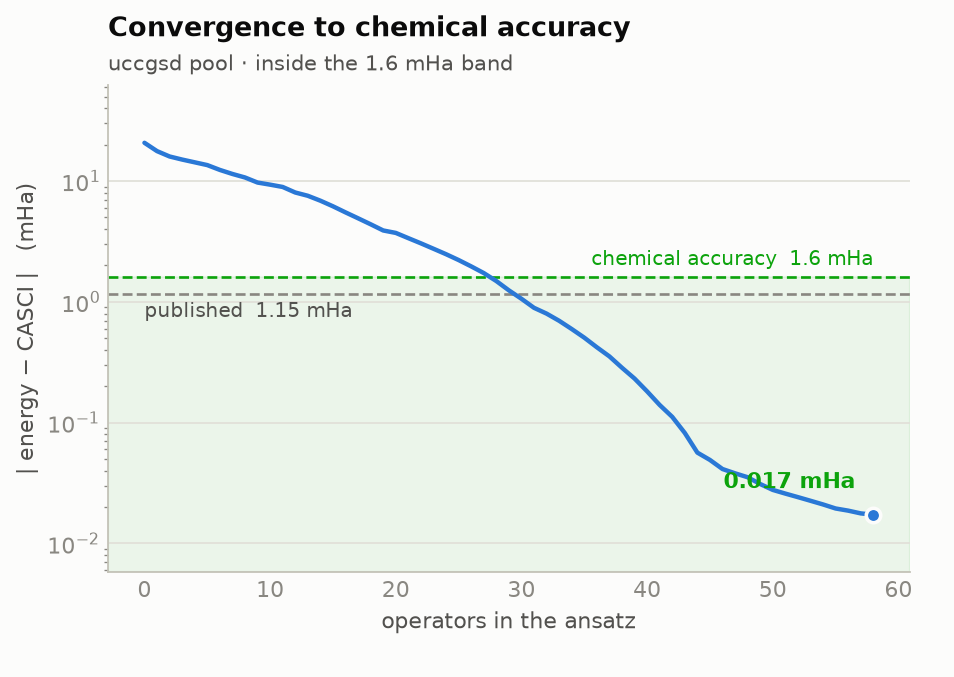
\includegraphics[width=0.66\textwidth]{figures/a-uccgsd-error.png}
\caption{Convergence of ADAPT-VQE with the UCCGSD pool. The error against the
exact active-space energy falls below chemical accuracy at 28 operators and
terminates at $0.017\mHa$. The published statevector result for the same active
space, $1.15\mHa$~\cite{koziell}, is marked for reference; the two are not
directly comparable, as discussed in Section~\ref{sec:A:published}.}
\label{fig:A:g:error}
\end{figure}

\begin{figure}[htbp]
\centering
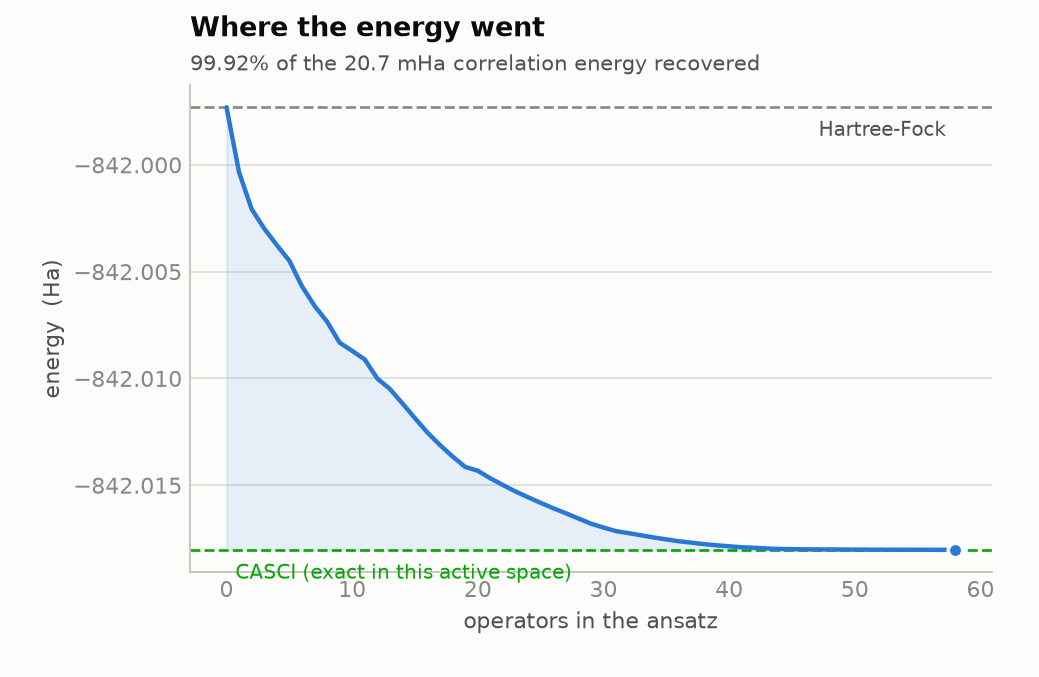
\includegraphics[width=0.66\textwidth]{figures/a-uccgsd-energy.png}
\caption{The same trajectory in absolute energy, from the Hartree--Fock
determinant to the exact active-space energy. The shaded region is the
$20.7\mHa$ of correlation energy available within CAS(6e,6o), of which $99.92\%$
is recovered.}
\label{fig:A:g:energy}
\end{figure}

\begin{figure}[htbp]
\centering
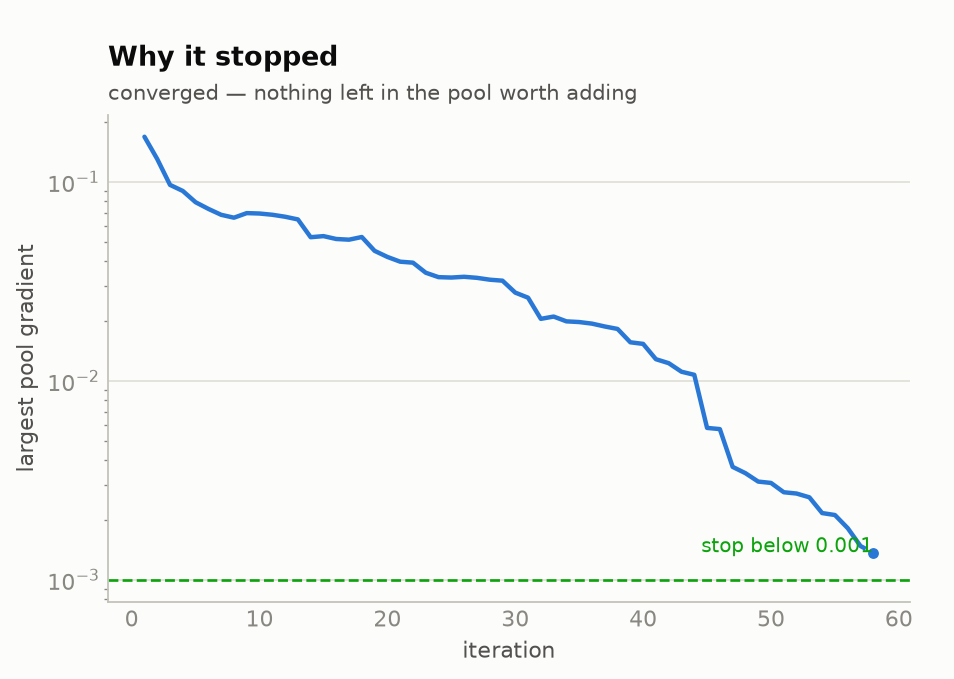
\includegraphics[width=0.66\textwidth]{figures/a-uccgsd-gradient.png}
\caption{The largest pool gradient at each iteration, which is the quantity
governing termination. The calculation stops when it falls below $10^{-3}$,
having exhausted the operators worth appending.}
\label{fig:A:g:grad}
\end{figure}

\begin{figure}[htbp]
\centering
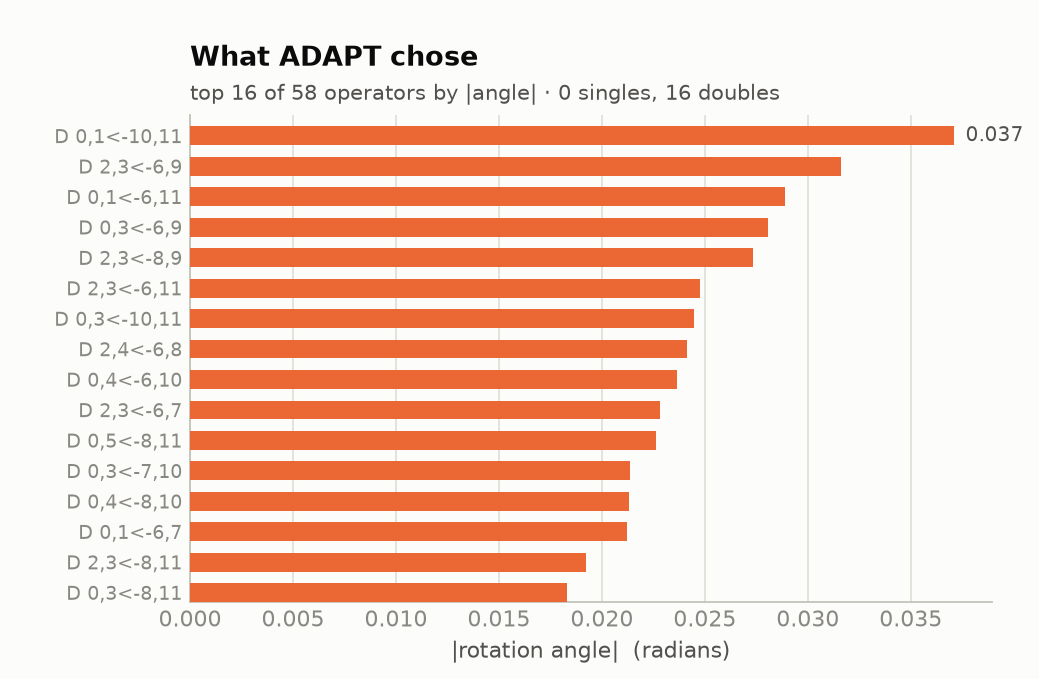
\includegraphics[width=0.72\textwidth]{figures/a-uccgsd-operators.png}
\caption{The sixteen largest rotation angles in the converged ansatz. All are
double excitations, and no single excitation appears anywhere in either ansatz.
This is expected for a closed-shell RHF reference, for which Brillouin's
theorem causes the singles gradients to vanish at the starting point.}
\label{fig:A:g:ops}
\end{figure}

\subsection{Coincidence of the two operator-selection trajectories}
\label{sec:A:trajectory}

Table~\ref{tab:A:results} invites the interpretation that the generalised pool
succeeds where the standard pool fails. The data exclude that interpretation.

Comparison of the two calculations step by step shows that, for all 31
iterations performed by both, the energies and pool gradients agree to better
than $10^{-12}$; they are the same values rather than similar ones. A sample of
the trajectory is given in Table~\ref{tab:A:trajectory}.

\begin{table}[htbp]
\centering
\small
\caption{The first 31 ADAPT iterations of the two calculations. Operator labels
differ only in the direction convention of the two pool enumerations
($\mathrm{D}\ 10{,}11 \leftarrow 0{,}1$ against
$\mathrm{D}\ 0{,}1 \leftarrow 10{,}11$); the operators, energies and gradients
are identical. Errors are against $-842.0180419414\Ha$.}
\label{tab:A:trajectory}
\begin{tabular}{@{}rrrr@{}}
\toprule
Iteration & Pool gradient & Energy (Ha) & Error (mHa) \\
\midrule
 1 & $1.687\times10^{-1}$ & $-842.000348871$ & 17.693 \\
 2 & $1.303\times10^{-1}$ & $-842.002070089$ & 15.972 \\
 3 & $9.661\times10^{-2}$ & $-842.002982864$ & 15.059 \\
 5 & $7.903\times10^{-2}$ & $-842.004488576$ & 13.553 \\
10 & $6.934\times10^{-2}$ & $-842.008708670$ &  9.333 \\
15 & $5.338\times10^{-2}$ & $-842.011863405$ &  6.179 \\
20 & $4.195\times10^{-2}$ & $-842.014322432$ &  3.720 \\
25 & $3.304\times10^{-2}$ & $-842.015825043$ &  2.217 \\
30 & $2.775\times10^{-2}$ & $-842.016982405$ &  1.060 \\
31 & $2.617\times10^{-2}$ & $-842.017150278$ &  0.892 \\
\midrule
\multicolumn{4}{@{}l}{\emph{Calculation 1 terminates here on its operator
budget. Calculation 2 continues:}} \\
\midrule
40 & $1.533\times10^{-2}$ & $-842.017860706$ &  0.181 \\
50 & $3.064\times10^{-3}$ & $-842.018014246$ &  0.028 \\
58 & $1.361\times10^{-3}$ & $-842.018024689$ &  0.017 \\
\bottomrule
\end{tabular}
\end{table}

The explanation is direct. UCCGSD contains UCCSD; the gradient ranking selected
the same operators, in the same order, from both pools; and the two
calculations were consequently identical until the first exhausted its budget.
The additional 372 double excitations available in the generalised pool
contributed nothing to the first 31 selections.

\begin{unsupported}[Not established: a comparison of operator pools]
No conclusion is drawn regarding UCCSD relative to UCCGSD. Such a comparison
requires both calculations to converge; the budgets here were 31 and 100, and
the first terminated on its budget with a gradient twenty times its threshold.
Reported as ``UCCSD yields $0.892\mHa$ and UCCGSD yields $0.017\mHa$'',
Table~\ref{tab:A:results} would support a conclusion contradicted by its own
underlying data. The decisive experiment is a single change of configuration:
repetition of the UCCSD calculation with a 100-operator budget. The expectation
is convergence to within a few hundredths of a millihartree of Calculation 2,
since 32 of its 63 operators were never offered.
\end{unsupported}

The same reasoning disposes of the contamination result. Because the states at
iteration 31 are the same state, the value $\Ssq = 2.8 \times 10^{-3}$ observed
there is not attributable to the UCCSD generator set; it is a property of a
truncated ADAPT ansatz, and continuation of the same trajectory reduces it by
three orders of magnitude. The practical consequence is that a partially
converged ADAPT ansatz may exhibit symmetry breaking while remaining on a
trajectory toward a symmetric state, so contamination measured before
convergence is not grounds for abandoning a pool.

Figure~\ref{fig:A:s:grad} records the termination of the truncated
calculation, and Figure~\ref{fig:A:s:error} its error trajectory.

\begin{figure}[htbp]
\centering
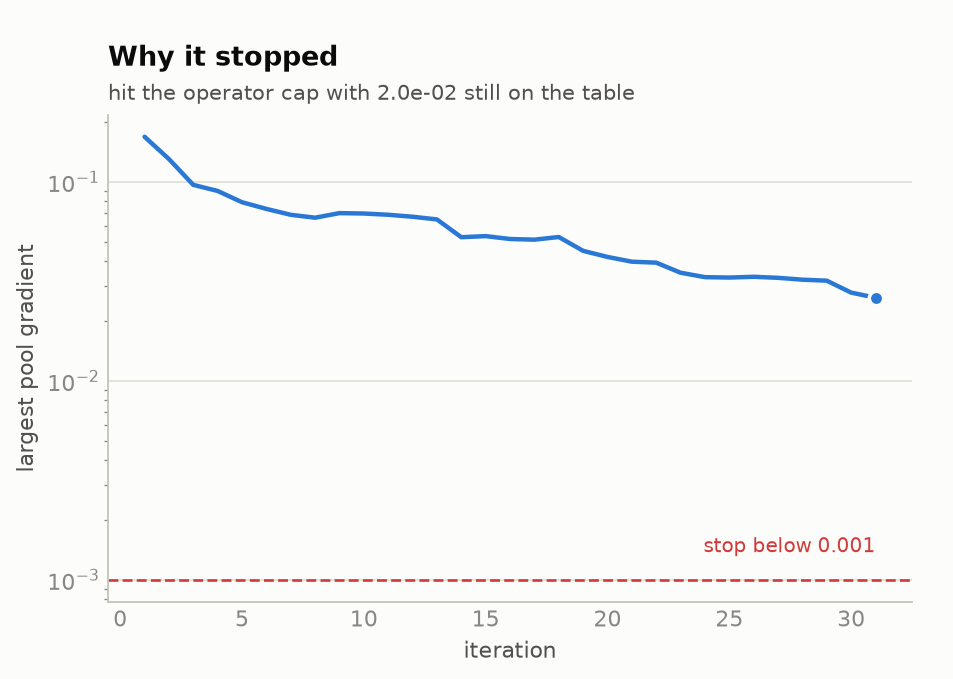
\includegraphics[width=0.66\textwidth]{figures/a-uccsd-gradient.png}
\caption{Termination of the truncated calculation. The pool gradient remains at
$2.0 \times 10^{-2}$ when the operator cap is reached, twenty times the
threshold that would have justified stopping. This panel, rather than the
energy, is the accurate summary of the calculation.}
\label{fig:A:s:grad}
\end{figure}

\begin{figure}[htbp]
\centering
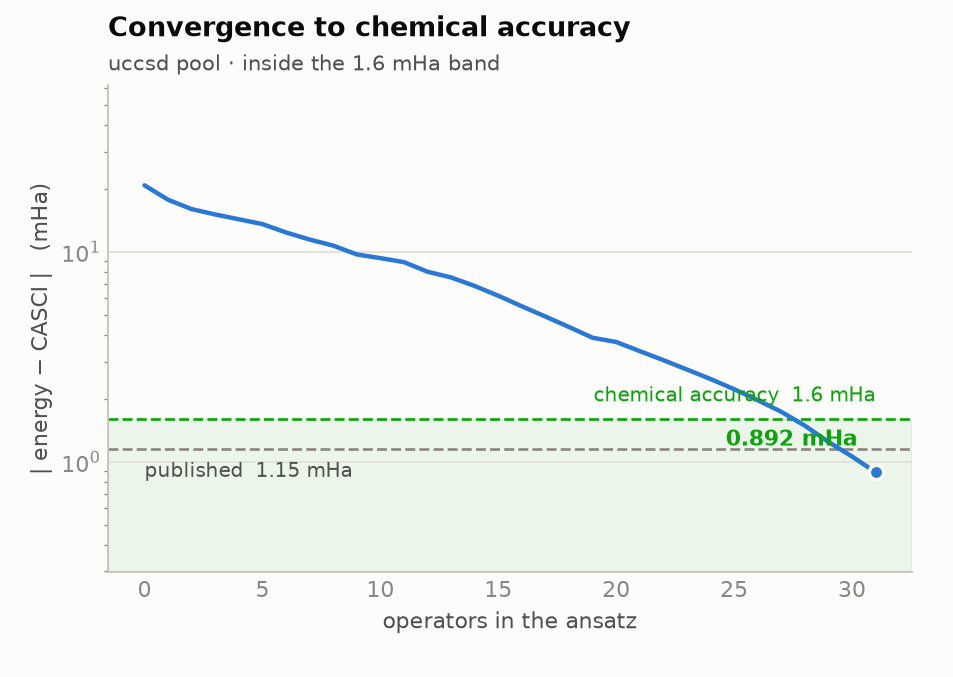
\includegraphics[width=0.66\textwidth]{figures/a-uccsd-error.png}
\caption{Error trajectory of the truncated calculation, terminating at
$0.892\mHa$. Over its common range this trajectory is numerically identical to
Figure~\ref{fig:A:g:error}, as established in
Section~\ref{sec:A:trajectory}.}
\label{fig:A:s:error}
\end{figure}

\subsection{Circuit resource requirements}

The converged ansatz, synthesised exactly and transpiled at optimisation level
3, requires 2988 two-qubit gates, 4674 single-qubit gates and a circuit depth
of 5296 on 12 qubits, for 58 variational parameters. At two-qubit error rates
presently attainable, a circuit of this depth does not return an energy of
$0.017\mHa$. The wall time of $133$~s reported in
Table~\ref{tab:A:results} is accordingly simulator time for a circuit that has
no current hardware realisation, and the comparison of the following section
should be read with that in mind.

\subsection{Classical baselines in the same active space}
\label{sec:A:classical}

MP2, CCSD and CCSD(T) were computed in the identical active space, with the
identical frozen core, from the identical integrals. Results are collected in
Table~\ref{tab:A:classical} and assessed against the criteria of
Section~\ref{sec:methods:criteria}.

\begin{table}[htbp]
\centering
\small
\caption{Imipramine CAS(6e,6o): all methods against the exact active-space
energy. The RHF calculation common to all methods required a further 92.5~s and
is excluded from every row. Wall times are indicative only; see
Section~\ref{sec:limitations}.}
\label{tab:A:classical}
\begin{tabular}{@{}lrrr@{}}
\toprule
Method & Energy (Ha) & Error (mHa) & Time (s) \\
\midrule
Hartree--Fock            & $-841.9973061558$ & 20.736 & --- \\
MP2                      & $-842.0102524898$ &  7.789 &   5.7 \\
ADAPT-VQE, 31 operators  & $-842.0171502782$ &  0.892 &  52.4 \\
CCSD                     & $-842.0180213368$ &  0.021 & 252.9 \\
ADAPT-VQE, 58 operators  & $-842.0180246890$ &  0.017 & 133.0 \\
\textbf{CCSD(T)}         & $-842.0180339214$ & \textbf{0.008} & 502.1 \\
CASCI (exact here)       & $-842.0180419414$ &  0     & --- \\
\bottomrule
\end{tabular}
\end{table}

CCSD(T) is more accurate than the converged quantum ansatz by a factor of two,
and CCSD is comparable to it. All three lie far within chemical accuracy.

\begin{result}[Established by Case A]
In an active space for which the exact result is computable, a converged
ADAPT-VQE ansatz is accurate to $0.017\mHa$ and is surpassed by CCSD(T). This
is a calibration result: it indicates that the quantum implementation is sound
and that the active space is too weakly correlated to require it.
\end{result}

\begin{unsupported}[Not established: that this ordering persists at larger scale]
The question of consequence is not which method is superior on 400
determinants, but whether the ordering survives into active spaces where CASCI
is unavailable. These data cannot address it. CCSD(T) is favoured here because
the reference determinant dominates, and its advantage is expected to erode
precisely where that ceases to hold, as it does along the \LiS{} coordinate,
where CCSD(T) degrades by three orders of magnitude and where ADAPT-VQE was not
computed. A single weakly correlated 12-qubit result is not evidence concerning
strongly correlated larger ones, in either direction. The decisive experiment
is inexpensive and the implementation already exists: ADAPT-VQE on the cached
\LiS{} Hamiltonian at $2.10$ and $6.00\Ang$, listed as item 2 of
Section~\ref{sec:unsupported}.
\end{unsupported}

\subsection{Comparison with the published study}
\label{sec:A:published}

The source study~\cite{koziell} reports, for imipramine CAS(6e,6o)/6-31G at 12
qubits with RHF orbitals and Jordan--Wigner mapping, a CASCI energy of
$-841.953249\Ha$, a statevector VQE energy of $-841.952101\Ha$ corresponding to
an error of $1.15\mHa$ obtained with ADAPT-GQE circuits, and a hardware energy
of $-841.752841\Ha$.

The total energies obtained here differ from those by approximately $65\mHa$
because a different conformer is used; the conformer of the source study is not
published. Total energies are therefore not comparable and are not compared.
The comparable quantity is each study's error against its own CASCI reference:
$1.15\mHa$ there against $0.017\mHa$ here. The difference is attributed to
ansatz expressiveness and convergence criteria rather than to implementation
quality, the circuits of the source study having been generated under a
hardware-executability constraint that did not apply here, at a resource cost
documented in the preceding section.

% ================================================================= CASE B ===
\section{Case B: \LiS, CAS(12e,12o), 24 qubits}
\label{sec:B}

\subsection{Molecular system and dissociation coordinate}

\LiS{} is treated in a linear Li--S--Li geometry with the STO-3G basis,
comprising 22 electrons in 19 orbitals. CAS(12e,12o) freezes the five lowest
orbitals and discards the two highest virtuals, giving 24 qubits and
$853{,}776$ determinants. The frozen set is verified to constitute the sulfur
$1s2s2p$ shell, whose orbitals lie near $-91$, $-9$ and $-6.7\Ha$ while no
other orbital lies below $-3\Ha$; the core--active gap is $3.88\Ha$ at
equilibrium.

The coordinate extends one Li--S bond while the second is held at $2.10\Ang$,
over thirteen geometries from $1.70$ to $6.00\Ang$. The reference at every
geometry is CASCI in the same active space.

Figure~\ref{fig:B:occ} indicates the character of the coordinate. At
$1.70\Ang$ the natural occupancies are near-integer. At $6.00\Ang$ three
orbitals carry fractional occupancy, approximately $1.03$, $1.63$ and $1.33$,
which is multireference character in its most direct expression.

\begin{figure}[htbp]
\centering
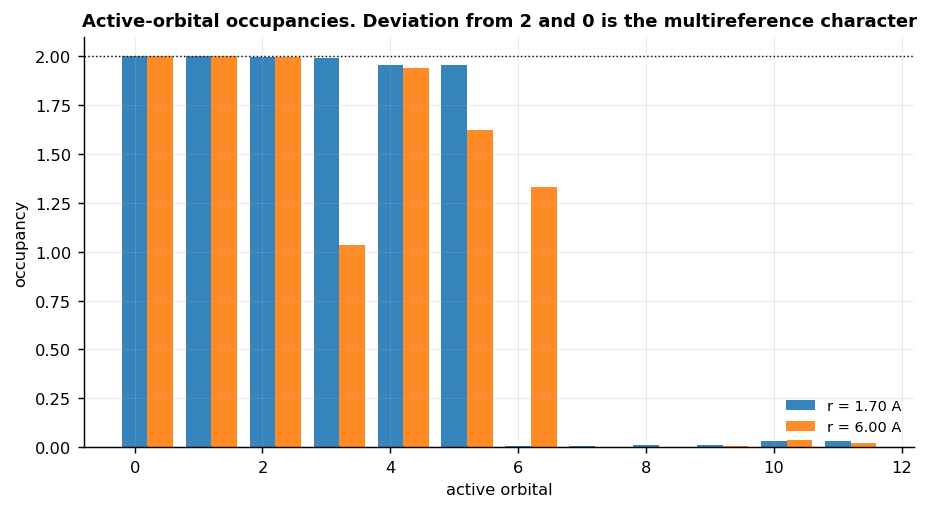
\includegraphics[width=0.70\textwidth]{figures/li2s-occupancies.png}
\caption{Active-orbital occupancies at the two extremes of the coordinate.
Deviation from 2 and 0 measures multireference character. At $1.70\Ang$ the
occupancies are nearly integer; at $6.00\Ang$ three orbitals are fractionally
occupied, a configuration that a single-reference method cannot represent.}
\label{fig:B:occ}
\end{figure}

\subsection{HI-VQE protocol}
\label{sec:B:protocol}

HI-VQE~\cite{hivqe} replaces the expectation-value measurement of a
conventional VQE~\cite{vqe} with a sampling step. A parameterised circuit is
sampled in the computational basis; the resulting bitstrings are interpreted as
electronic configurations; these, together with configurations proposed by a
classical single-and-double expansion, define a subspace; the Hamiltonian is
projected onto that subspace and diagonalised exactly; and the resulting energy
and its gradient with respect to the circuit parameters drive the subsequent
iteration. Structurally, the classical component is a selected-CI procedure in
the tradition of CIPSI~\cite{cipsi} and SHCI~\cite{shci}, with the circuit
supplying part of the selection. This observation is returned to in
Section~\ref{sec:B:ablation}, since it determines how demanding the classical
control is.

The consequence for measurement cost is the motivation for the method. A
conventional VQE applied to this Hamiltonian requires $15{,}697$ Pauli words
per energy evaluation, whereas HI-VQE requires one measurement setting, since
it requires configurations rather than expectation values
(Figure~\ref{fig:B:cost:m}). The circuit itself is modest by comparison with
the ADAPT ansatz of Case~A (Figure~\ref{fig:B:cost:c}).

\begin{figure}[htbp]
\centering
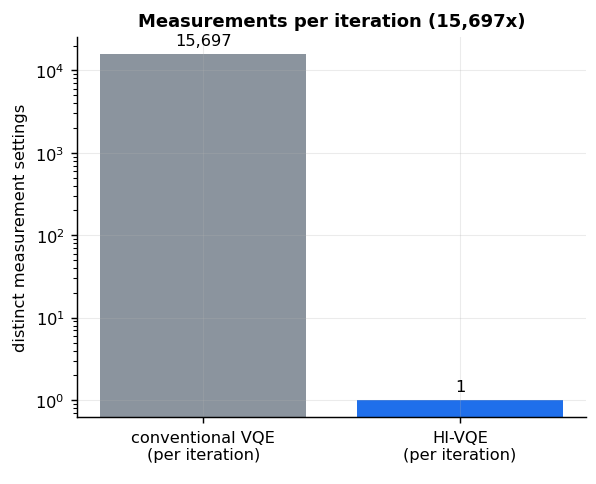
\includegraphics[width=0.56\textwidth]{figures/b-cost-measurement.png}
\caption{Distinct measurement settings required per iteration: $15{,}697$ Pauli
words for a conventional VQE on this Hamiltonian, against a single
computational-basis setting for HI-VQE.}
\label{fig:B:cost:m}
\end{figure}

\begin{figure}[htbp]
\centering
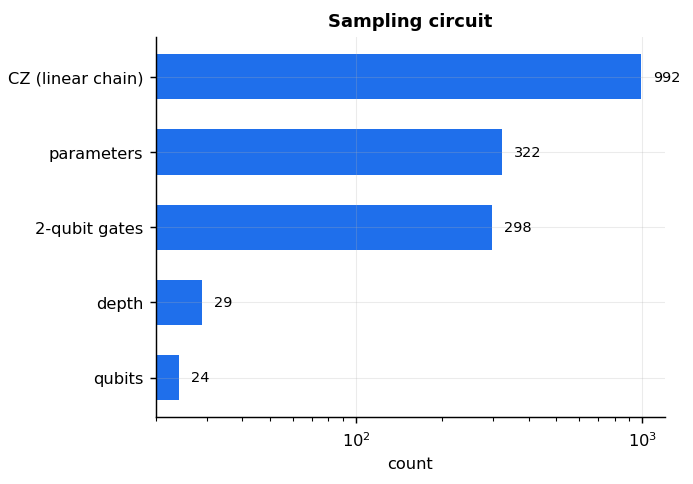
\includegraphics[width=0.62\textwidth]{figures/b-cost-circuit.png}
\caption{Resources of the sampling circuit, a hardware-efficient unitary
cluster Jastrow comprising nearest-neighbour Givens rotations within each spin
block and a number--number Jastrow layer coupling them. Every gate commutes
with both spin-resolved number operators, so that on a noiseless simulator each
shot is a valid configuration and particle-number leakage is identically zero
rather than merely small.}
\label{fig:B:cost:c}
\end{figure}

The variational structure of the method is essential to
Section~\ref{sec:B:void}. Every reported energy is the lowest eigenvalue of
$PHP$ for the projector $P$ onto the current subspace, and is therefore an
upper bound on the ground state of whichever symmetry sector the sampled
configurations span, for any $P$. Noise in the sampler can only propose an
inferior subspace; it cannot bias the energy downward.

Parameters are as follows: subspace capped at $20{,}000$ determinants;
classical expansion of 400 candidates per iteration generated from the eight
leading configurations; amplitude screening at $10^{-6}$; second-order
perturbative ranking; 8192 shots; one circuit repetition; SPSA optimisation;
convergence at $10^{-6}\Ha$ sustained over five iterations; random seed 1234.
Complete settings are given in Appendix~\ref{app:settings}.

\subsection{Dissociation curve}

The complete set of geometries is given in Table~\ref{tab:B:curve}, and the
curve is shown against the classical hierarchy in
Figures~\ref{fig:B:curve} and~\ref{fig:B:curve:err}.

\begin{table}[htbp]
\centering
\small
\caption{\LiS{} dissociation, CAS(12e,12o)/STO-3G, 24 qubits. Errors are
against CASCI in the same active space. The two italicised rows are void: the
reference at those geometries is not the sector ground state
(Section~\ref{sec:B:void}), so no method's error there is interpretable.}
\label{tab:B:curve}
\begin{tabular}{@{}rrrrrrrr@{}}
\toprule
$r$ (\AA) & $E$(HF) & $E$(HI-VQE) & $E$(CASCI) & err (mHa) & HF err (mHa) & dets & \% space \\
\midrule
1.700 & $-407.950117$ & $-407.985509$ & $-407.985607$ & $+0.099$ & 35.5 & 19{,}992 & 2.342 \\
1.900 & $-407.964402$ & $-408.001987$ & $-408.002076$ & $+0.089$ & 37.7 & 19{,}950 & 2.337 \\
2.000 & $-407.960694$ & $-407.999205$ & $-407.999309$ & $+0.104$ & 38.6 & 19{,}992 & 2.342 \\
2.100 & $-407.952748$ & $-407.992132$ & $-407.992208$ & $+0.076$ & 39.5 & 19{,}932 & 2.335 \\
2.200 & $-407.942002$ & $-407.982123$ & $-407.982225$ & $+0.102$ & 40.2 & 19{,}966 & 2.339 \\
2.400 & $-407.915865$ & $-407.957314$ & $-407.957425$ & $+0.111$ & 41.6 & 19{,}881 & 2.329 \\
2.600 & $-407.887294$ & $-407.929953$ & $-407.930087$ & $+0.134$ & 42.8 & 19{,}881 & 2.329 \\
2.900 & $-407.844982$ & $-407.884942$ & $-407.885013$ & $+0.071$ & 40.0 & 19{,}880 & 2.328 \\
\midrule
\emph{3.200} & \emph{$-407.806559$} & \emph{$-407.862021$} & \emph{$-407.853522$} & \emph{void} & --- & 19{,}881 & 2.329 \\
\emph{3.600} & \emph{$-407.764023$} & \emph{$-407.849591$} & \emph{$-407.825353$} & \emph{void} & --- & 19{,}881 & 2.329 \\
\midrule
4.200 & $-407.719485$ & $-407.840669$ & $-407.840733$ & $+0.065$ & 121.2 & 19{,}881 & 2.329 \\
5.000 & $-407.686955$ & $-407.837262$ & $-407.837292$ & $+0.030$ & 150.3 & 19{,}880 & 2.328 \\
6.000 & $-407.668269$ & $-407.836424$ & $-407.836433$ & $+0.009$ & 168.2 & 11{,}118 & 1.302 \\
\bottomrule
\end{tabular}
\end{table}

Across the eleven valid geometries the largest error is $0.134\mHa$, a factor
of twelve within chemical accuracy, and the smallest is $0.009\mHa$.
Hartree--Fock errs by $35.5$ to $168.2\mHa$ over the same points.

The derived quantity of Table~\ref{tab:B:derived} constitutes a more stringent
test than any individual total energy, a dissociation energy being a difference
in which the systematic component of the error cancels.

\begin{table}[htbp]
\centering
\small
\caption{Quantities derived from the dissociation curve.}
\label{tab:B:derived}
\begin{tabular}{@{}lrr@{}}
\toprule
& HI-VQE & CASCI \\
\midrule
Minimum on this grid & $1.900\Ang$ & $1.900\Ang$ \\
Dissociation energy to the final point & 103.89 kcal\,mol$^{-1}$ & 103.94 kcal\,mol$^{-1}$ \\
Error in the dissociation energy & \multicolumn{2}{r}{0.051 kcal\,mol$^{-1}$} \\
\bottomrule
\end{tabular}
\end{table}

\begin{figure}[htbp]
\centering
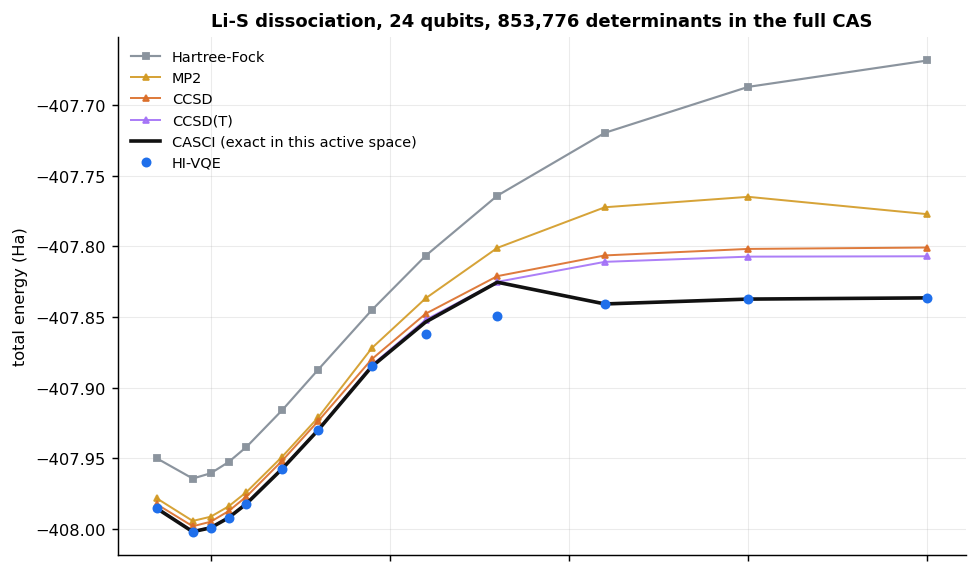
\includegraphics[width=0.76\textwidth]{figures/b-curve.png}
\caption{The Li--S dissociation curve, with the classical hierarchy shown
against CASCI and HI-VQE points overlaid. The reference curve falls between
$3.6$ and $4.2\Ang$; a dissociation curve cannot do so, and this observation
constitutes the second argument of Section~\ref{sec:B:void}.}
\label{fig:B:curve}
\end{figure}

\begin{figure}[htbp]
\centering
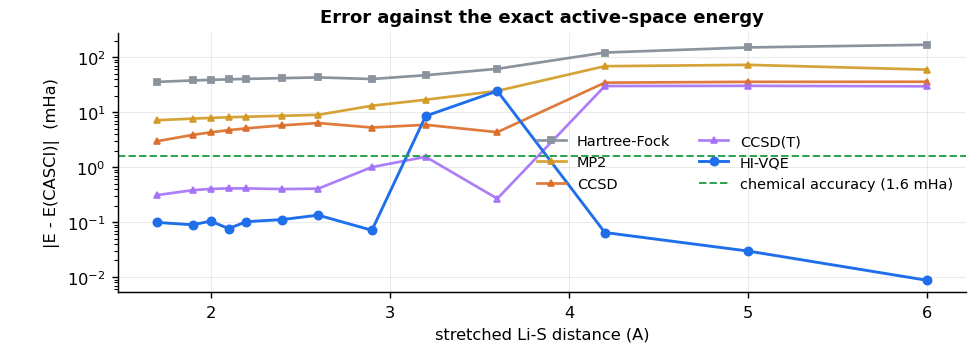
\includegraphics[width=0.76\textwidth]{figures/b-curve-error.png}
\caption{Absolute error against CASCI on a logarithmic scale. Two features
determine the remainder of this section: the excursion in the HI-VQE error at
$3.2$ and $3.6\Ang$, which reflects failure of the reference rather than of the
method (Section~\ref{sec:B:void}); and the step in the classical curves between
$3.6$ and $4.2\Ang$, which coincides with a change of spin sector
(Section~\ref{sec:B:sector}).}
\label{fig:B:curve:err}
\end{figure}

\subsection{Invalidity of the reference at two geometries}
\label{sec:B:void}

At $r = 3.20$ and $3.60\Ang$ the reported errors are $-8.499$ and
$-24.238\mHa$. An energy below the reference is not a superior result; in a
correct variational calculation it is not attainable. The workflow labels both
\code{INCONSISTENT} rather than reporting them.

\textbf{First argument, from the variational bound.} The HI-VQE energy is the
lowest eigenvalue of $PHP$, and the sampling circuit commutes with both
spin-resolved number operators, so the sampled configurations do not leave the
$S_z = 0$ sector. Consequently

\[
E_{\text{HI-VQE}} \;\geq\; \min_{\psi \,\in\, S_z = 0}
\frac{\langle \psi | H | \psi \rangle}{\langle \psi | \psi \rangle}
\;=\; E_0(S_z = 0).
\]

If $E_{\text{HI-VQE}} < E_{\text{CASCI}}$ then $E_{\text{CASCI}} > E_0(S_z=0)$,
and the reference is not the ground state of the sector it was intended to
diagonalise. The inequality admits only this direction, so the conclusion
concerns the reference and not the method.

\textbf{Second argument, from the shape of the curve.} A dissociation curve
increases monotonically toward its asymptote. The reference does not:

\begin{center}
\small
\begin{tabular}{@{}lrrrr@{}}
\toprule
$r$ (\AA) & 3.200 & 3.600 & 4.200 & 6.000 (asymptote) \\
\midrule
CASCI  & $-407.853522$ & $-407.825353$ & $-407.840733$ & $-407.836433$ \\
HI-VQE & $-407.862021$ & $-407.849591$ & $-407.840669$ & $-407.836424$ \\
\bottomrule
\end{tabular}
\end{center}

The reference increases from $3.2$ to $3.6\Ang$ and then decreases by
$15.4\mHa$ at $4.2\Ang$, its value at $3.6\Ang$ lying above its own asymptote.
The HI-VQE curve increases monotonically to the asymptote throughout. Two
independent arguments identify the same two geometries.

\textbf{Mechanism.} PySCF dispatches a closed-shell RHF reference to
\code{direct\_spin0}, which exploits the $\alpha \leftrightarrow \beta$
symmetry of the CI matrix. This is a legitimate optimisation and is
inappropriate here: a CI vector constrained to be symmetric under that exchange
spans only the even-$S$ states, so the solver cannot return a triplet even
where the triplet is the ground state. The solver was changed to
\code{direct\_spin1}, which imposes only $S_z$, this being the constraint under
which HI-VQE itself operates, and the Davidson convergence was tightened to
$10^{-12}$, since the near-degeneracy motivating the change also degrades
convergence of the final digits.

\begin{caution}[The correction is incomplete and is reported as such]
Following the change the reference correctly returns $\Ssq \approx 2$ from
$4.20\Ang$ onward. At $3.20$ and $3.60\Ang$ it continues to return a singlet.
The probable explanation is convergence of the Davidson procedure onto an
excited root in a region of near-degeneracy; the diagnostic experiment is a
multi-root CASCI calculation at those two geometries, which was not performed.
Until it is, both geometries constitute an open defect and all errors there are
void, for the classical methods of Table~\ref{tab:B:classical} equally as for
HI-VQE.
\end{caution}

\subsection{Spin sector along the coordinate}
\label{sec:B:sector}

The diagnostic quantity throughout is $\Ssq$, recorded for both the returned
state and the reference (Table~\ref{tab:B:spin}).

\begin{table}[htbp]
\centering
\small
\caption{Spin expectation values along the coordinate. The reference changes
sector between $3.60$ and $4.20\Ang$, whereas HI-VQE reaches the triplet from
$3.20\Ang$. The two geometries at which they disagree are precisely the two
void geometries.}
\label{tab:B:spin}
\begin{tabular}{@{}rrrl@{}}
\toprule
$r$ (\AA) & $\Ssq$ (HI-VQE) & $\Ssq$ (reference) & Classification \\
\midrule
2.900 & $1.0\times10^{-4}$ & $2.5\times10^{-14}$ & \code{CHEMICAL ACCURACY} \\
3.200 & $2.0000$           & $8.0\times10^{-15}$ & \code{INCONSISTENT} \\
3.600 & $1.9997$           & $2.1\times10^{-14}$ & \code{INCONSISTENT} \\
4.200 & $1.9984$           & $2.0000$            & \code{SPIN CONTAMINATED} \\
5.000 & $1.9896$           & $1.9850$            & \code{SPIN CONTAMINATED} \\
6.000 & $1.0002$           & $1.9467$            & \code{SPIN CONTAMINATED} \\
\bottomrule
\end{tabular}
\end{table}

The underlying physics is standard. At a dissociated Li--S bond the fragments
are Li($^2$S) and LiS($^2\Pi$), two doublets whose singlet and triplet
couplings become degenerate; which lies lower is a genuine question whose
answer changes along the coordinate. The crossing occurs between $2.90$ and
$3.20\Ang$, HI-VQE returning $\Ssq \approx 2$ from $3.20\Ang$ onward.

At $6.00\Ang$ the two values differ again, $1.00$ against $1.95$, yet the
energies agree to $0.009\mHa$. This combination is the signature of genuine
degeneracy: for two non-interacting doublets the singlet and triplet couplings
are isoenergetic, so an equal mixture, for which $\Ssq = 1$, and a nearly pure
triplet are both ground states, and no energy can distinguish them. This is the
reason $\Ssq$ is reported alongside every energy rather than inferred from it.

The consequence for the classical baselines is the third instance of the
failure mode, and the least apparent.

\begin{result}[Result 4, stated precisely]
MP2, CCSD and CCSD(T) as computed here are constructed on the closed-shell RHF
determinant and are therefore singlet-constrained. From $4.20\Ang$ onward the
reference against which they are scored has $\Ssq \approx 2$. Their reported
errors at those geometries are consequently a sum of a spin-sector difference
and a correlation-treatment deficiency, and these data cannot separate the two
contributions. The step from $0.27\mHa$ at $3.60\Ang$ to $29.83\mHa$ at
$4.20\Ang$ is indicative precisely because $T_1$ increases smoothly across the
same interval, from $0.0896$ to $0.1134$: an error increasing by two orders of
magnitude while its presumed cause changes by $27\%$ is not attributable to
that quantity alone.
\end{result}

One geometry admits the decomposition. At $6.00\Ang$ the singlet and triplet
are degenerate, as the $0.009\mHa$ agreement above demonstrates, so the sector
contribution vanishes and the entire $29.48\mHa$ CCSD(T) error is a
correlation-treatment deficiency: the established breakdown of an RHF-based
coupled-cluster treatment at dissociation, corroborated by $T_1 = 0.1216$ and
by the fractional occupancies of Figure~\ref{fig:B:occ}. At $4.20$ and
$5.00\Ang$ no such argument is available and none is attempted.

\subsection{Subspace compression and convergence}

The method attains these accuracies within $2.3\%$ of the determinant space,
and within $1.3\%$ at $6.00\Ang$. The strongly correlated geometry requires
fewer determinants, since at full dissociation the wavefunction is dominated by
a small number of fragment configurations. Both quantities are shown by
iteration in Figures~\ref{fig:B:conv:e} and~\ref{fig:B:conv:d}.

\begin{figure}[htbp]
\centering
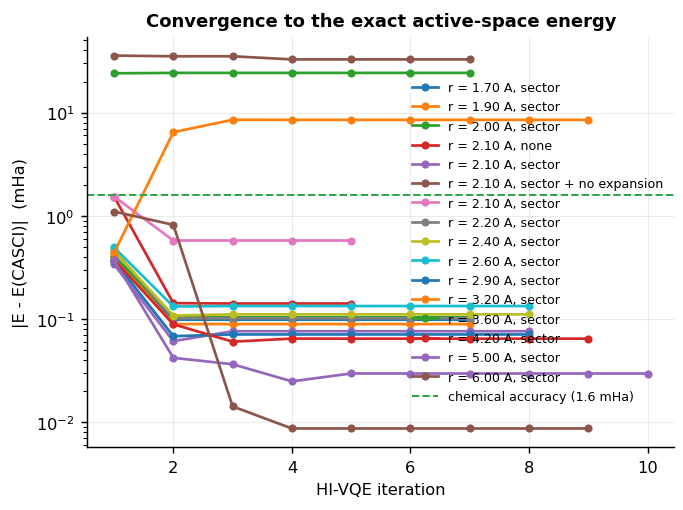
\includegraphics[width=0.62\textwidth]{figures/b-conv-error.png}
\caption{Error against CASCI by iteration for all calculations. Most geometries
converge by the fourth iteration and all are stationary by the eighth. The two
trajectories plateauing above $8\mHa$ are the void geometries of
Section~\ref{sec:B:void}; the trajectory near $30\mHa$ is the no-expansion
ablation.}
\label{fig:B:conv:e}
\end{figure}

\begin{figure}[htbp]
\centering
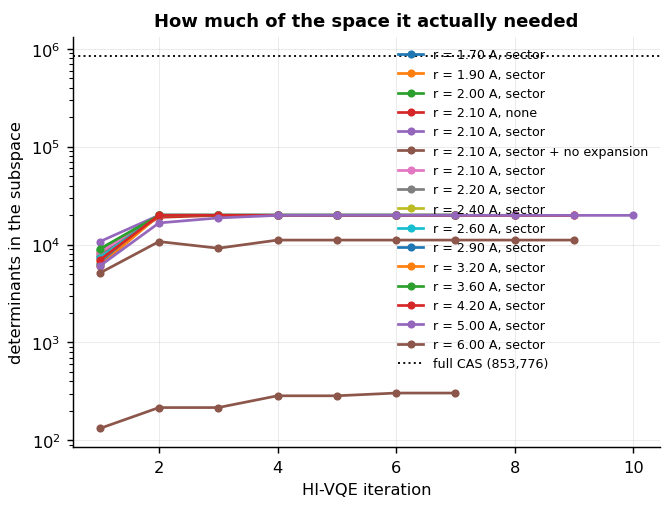
\includegraphics[width=0.62\textwidth]{figures/b-conv-dets.png}
\caption{Determinants in the subspace by iteration, against the full CAS
dimension of $853{,}776$. The subspace saturates at the $20{,}000$ cap within
two iterations for all production calculations; the trajectory near $3 \times
10^{2}$ is the circuit-only ablation, which never populates a usable subspace.}
\label{fig:B:conv:d}
\end{figure}

\subsection{Ablation of the algorithmic components}
\label{sec:B:ablation}

Three configurations were computed at $r = 2.10\Ang$: the complete method
(\code{sector}); the method with no circuit, the classical expansion proposing
every configuration (\code{none}), which is a conventional selected-CI and
constitutes the control of interest; and the circuit alone with the classical
expansion removed (\code{no expansion}).

\begin{table}[htbp]
\centering
\small
\caption{Ablation at $r = 2.10\Ang$: identical geometry, Hamiltonian,
determinant cap and convergence criteria. One calculation per configuration at
seed 1234.}
\label{tab:B:ablation}
\begin{tabular}{@{}lrrl@{}}
\toprule
Configuration & Error (mHa) & Determinants & Classification \\
\midrule
Complete method (\code{sector})    & 0.076 & 19{,}932 & \code{CHEMICAL ACCURACY} \\
Classical control (\code{none})    & 0.141 & 19{,}890 & \code{CHEMICAL ACCURACY} \\
Published expansion rule           & 0.576 & 19{,}881 & \code{CHEMICAL ACCURACY} \\
Circuit only (\code{no expansion}) & 32.745 &    304  & \code{SPIN CONTAMINATED} \\
\bottomrule
\end{tabular}
\end{table}

Two statements survive this table and one does not.

\textbf{Established.} The classical expansion is necessary. Its removal costs a
factor of $230$ in error and reduces the subspace from $19{,}932$ determinants
to $304$; no plausible seed-to-seed variation spans that interval.

\textbf{Established.} The classical expansion is sufficient at this geometry.
The control attains $0.141\mHa$, an order of magnitude within chemical
accuracy, with no quantum circuit. This is unsurprising given the nature of the
classical component, which is a selected-CI procedure; the selected-CI
literature~\cite{cipsi,shci} reports near-FCI accuracy on spaces substantially
larger than $853{,}776$ determinants.

\begin{unsupported}[Not established: that the circuit improves upon the control]
The complete method's $0.076\mHa$ against the control's $0.141\mHa$ is a factor
of $1.9$ obtained from one realisation of each, both stochastic, both at a
single seed, and both an order of magnitude within the acceptance threshold. No
variance estimate is available and there is accordingly no basis for treating
this as a difference. Three to five seeds at this geometry would resolve it.
\end{unsupported}

\begin{caution}[A figure in the generated output is misleading and is reproduced only to be withdrawn]
Figure~\ref{fig:B:ablation} plots mean error by configuration across all
calculations. Its \code{sector} bar lies at $2.44\mHa$ and appears inferior to
the $0.141\mHa$ control, which would invert even the weak reading above. This
is an artefact: that mean is taken over 14 calculations including the two void
geometries of Section~\ref{sec:B:void}, whose values of $-8.5$ and $-24.2\mHa$
dominate the average, whereas \code{none} comprises a single calculation at a
single geometry. Averaging over a defective reference does not constitute a
comparison. Table~\ref{tab:B:ablation} supersedes the figure.
\end{caution}

\begin{figure}[htbp]
\centering
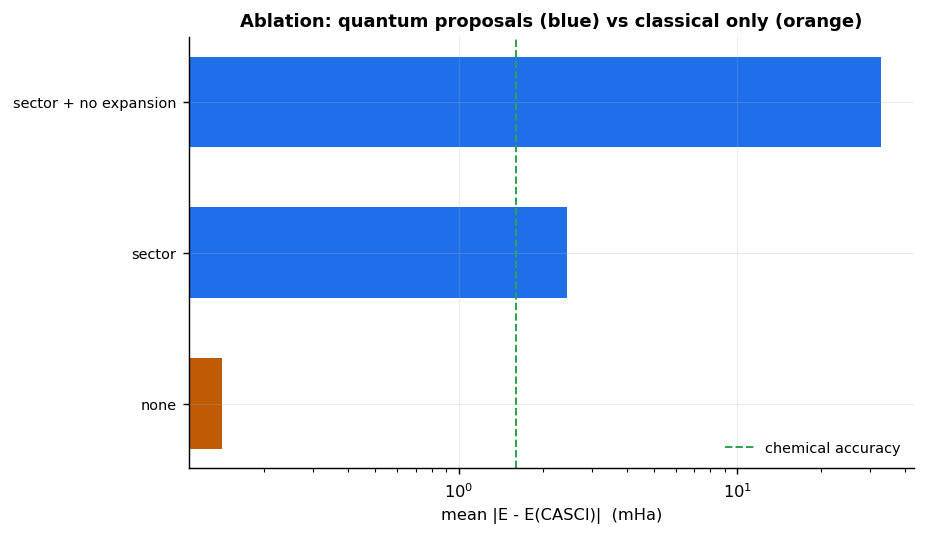
\includegraphics[width=0.60\textwidth]{figures/li2s-ablation.png}
\caption{Mean error by ablation configuration, as emitted by the reporting
code. This figure is not a result; see the preceding caution. Its \code{sector}
mean is contaminated by the two geometries at which the reference, rather than
the method, failed.}
\label{fig:B:ablation}
\end{figure}

\subsection{Classical baselines in the same active space}
\label{sec:B:classical}

\begin{table}[htbp]
\centering
\small
\caption{Classical baselines against CASCI, with the $T_1$
diagnostic~\cite{t1}. The rows at $3.200$ and $3.600\Ang$ are void for every
method (Section~\ref{sec:B:void}). From $4.200\Ang$ the reference is a triplet
while these methods are singlet-constrained, so those errors combine a
spin-sector difference with a correlation deficiency; only at $6.000\Ang$,
where the two spin states are degenerate, is the error unambiguously
correlation (Section~\ref{sec:B:sector}).}
\label{tab:B:classical}
\begin{tabular}{@{}rrrrrrl@{}}
\toprule
$r$ (\AA) & MP2 err & CCSD err & CCSD(T) err & HI-VQE err & $T_1$ & Ref.\ $\Ssq$ \\
 & (mHa) & (mHa) & (mHa) & (mHa) & & \\
\midrule
1.700 & $+7.11$  & $+2.95$  & $+0.31$  & $+0.099$ & 0.0239 & 0 \\
1.900 & $+7.62$  & $+3.86$  & $+0.38$  & $+0.089$ & 0.0270 & 0 \\
2.000 & $+7.85$  & $+4.29$  & $+0.40$  & $+0.104$ & 0.0287 & 0 \\
2.100 & $+8.06$  & $+4.70$  & $+0.41$  & $+0.076$ & 0.0304 & 0 \\
2.200 & $+8.25$  & $+5.08$  & $+0.41$  & $+0.102$ & 0.0321 & 0 \\
2.400 & $+8.58$  & $+5.75$  & $+0.40$  & $+0.111$ & 0.0354 & 0 \\
2.600 & $+8.93$  & $+6.34$  & $+0.41$  & $+0.134$ & 0.0387 & 0 \\
2.900 & $+13.08$ & $+5.24$  & $+1.00$  & $+0.071$ & 0.0509 & 0 \\
\midrule
\emph{3.200} & \emph{void} & \emph{void} & \emph{void} & \emph{void} & 0.0625 & 0 \\
\emph{3.600} & \emph{void} & \emph{void} & \emph{void} & \emph{void} & 0.0896 & 0 \\
\midrule
4.200 & $+68.50$ & $+34.37$ & $+29.83$ & $+0.065$ & 0.1134 & 2.000 \\
5.000 & $+72.45$ & $+35.54$ & $+30.06$ & $+0.030$ & 0.1197 & 1.985 \\
6.000 & $+59.30$ & $+35.67$ & $+29.48$ & $+0.009$ & 0.1216 & 1.947 \\
\bottomrule
\end{tabular}
\end{table}

Below the void interval CCSD(T) maintains errors of $0.3$ to $1.0\mHa$ and lies
within chemical accuracy at every geometry, HI-VQE being superior by a factor
of three to ten, which is a real but not decisive margin. At $6.00\Ang$, the
one dissociated geometry at which the comparison is unambiguous, CCSD(T) errs
by $29.48\mHa$, eighteen times chemical accuracy, against $0.009\mHa$ for
HI-VQE, a factor of $3.4 \times 10^{3}$.

\begin{result}[Established by Case B]
At $6.00\Ang$, where the reference is verified, the spin states are degenerate
and the comparison is therefore unambiguous, HI-VQE reproduces the exact
active-space energy to $0.009\mHa$ while sampling $1.3\%$ of the determinant
space, whereas the best classical method available in the same space errs by
$29.48\mHa$. This is a genuine three-order-of-magnitude result against coupled
cluster and is the strongest single quantity reported here.
\end{result}

\begin{unsupported}[Not established: that the quantum component is responsible]
The comparison above is between HI-VQE and coupled cluster, not between HI-VQE
and its own classical component. The \code{none} control was computed at
$2.10\Ang$ only, where it attained chemical accuracy unaided. Since that
control is a selected-CI procedure, and selected-CI is by construction a
multireference method, the reasonable expectation is that it also performs well
at $6.00\Ang$, possibly as well as the complete method. Were that so, the
correct conclusion would be that a classical selected-CI surpasses CCSD(T) by
three orders of magnitude at dissociation and that the circuit contributes
little, which is a materially different result. Computation of \code{none} at
$4.20$, $5.00$ and $6.00\Ang$ would decide the matter. It requires no PySCF,
only the cached Hamiltonians, and is the single most valuable experiment not
performed.
\end{unsupported}

\subsection{Comparison with the published study}

The source study~\cite{hivqe} fixes the active space, the reference method, the
algorithm and the nature of the coordinate. It does not report a geometry,
per-geometry energies or an orbital set, and does not specify the sampling
circuit. Total energies are therefore not reproducible from it and no such
claim is made. The comparable quantities, and those measured here, are the
error against the present CASCI reference at each geometry, the fraction of the
determinant space required, and the shape of the curve.

% ============================================================== DISCUSSION ==
\section{Discussion}
\label{sec:discussion}

\subsection{A common failure mode}

The three defects described above appear unrelated: a comparison of ansätze, a
reference energy, and a set of classical baselines. They are the same defect.

\begin{table}[htbp]
\centering
\small
\caption{One failure mode in three instances. In each, a plausible quantity was
produced by comparing states that were not comparable, and in each the
diagnostic that identified it was inexpensive.}
\label{tab:S:three}
\begin{tabular}{@{}p{2.7cm}p{4.4cm}p{3.2cm}p{3.4cm}@{}}
\toprule
Location & Quantities compared & Appearance & Diagnostic \\
\midrule
Case A,
\S\ref{sec:A:trajectory} &
Two operator pools, the calculations coinciding for 31 iterations and differing
only in budget &
A pool comparison, $0.892$ against $0.017\mHa$ &
Comparison of trajectories rather than endpoints \\[4pt]
Case B,
\S\ref{sec:B:void} &
A CASCI reference against a variationally bounded method in the same sector &
A method error of $-24\mHa$ &
Sign of the error; monotonicity of the curve \\[4pt]
Case B,
\S\ref{sec:B:sector} &
Singlet-constrained coupled cluster against a triplet reference &
A correlation discontinuity between $3.6$ and $4.2\Ang$ &
Recording $\Ssq$ of the reference \\
\bottomrule
\end{tabular}
\end{table}

The common structure is that each produced a quantity of the expected
magnitude. None resembled a numerical fault. The first two would have been
reported as results; the third would have been reported as the principal
finding.

\subsection{A variationally bounded method as a certificate on its reference}
\label{sec:discussion:certificate}

The detection described in Section~\ref{sec:B:void} was not fortunate. It is an
instance of a property that any variationally bounded method possesses, and
which is worth stating in general form because it inverts the customary
relationship between a quantum calculation and the classical reference used to
judge it.

Let $\mathcal{S}$ denote a symmetry sector, here $S_z = 0$, and let a method
return $E_{\text{q}} = \min \operatorname{spec}(PHP)$ for some projector $P$
onto a subspace of $\mathcal{S}$. Then $E_{\text{q}} \geq E_0(\mathcal{S})$ for
every $P$, with no assumption whatever on how $P$ was obtained. Consequently,
for any reference energy $E_{\text{ref}}$ asserted to equal
$E_0(\mathcal{S})$,

\[
E_{\text{q}} < E_{\text{ref}}
\quad\Longrightarrow\quad
E_{\text{ref}} > E_0(\mathcal{S}),
\]

that is, the assertion is false. The implication runs in one direction only,
which is precisely what makes it useful: a violation is not evidence of a
superior quantum result and cannot be produced by sampling noise, an
underconverged circuit or a poor choice of subspace, since all of these can
only raise $E_{\text{q}}$. The only remaining explanation is that the reference
is not the sector ground state.

Three features make this practical. The test costs nothing beyond the sign of a
quantity already computed. It requires no knowledge of the exact answer, which
is the regime in which references are least trustworthy. And it is not specific
to HI-VQE: sample-based diagonalisation and classical selected-CI share the
same bound, so the same certificate is available to any of them.

The customary hierarchy places the classical reference in judgement over the
quantum result. Where the quantum method carries a variational bound and the
reference does not carry a proof of convergence, the direction of inference is
the reverse of the customary one. In this study the CASCI reference at $3.20$
and $3.60\Ang$ was produced by a solver whose default restricted it to even-$S$
states, and no diagnostic internal to that calculation reported a difficulty:
it converged, and returned a plausible energy. What identified the defect was
a quantum calculation being scored against it.

\begin{result}[A recommended check]
Where a reference is obtained from an iterative eigensolver and a variationally
bounded method is available in the same sector, the sign of the error is a
convergence diagnostic for the reference and should be recorded as such.
Sustained negative errors indicate a reference defect and not a method success.
The corresponding positive statement is weaker but still useful: a positive
error confirms only that the reference lies below the method, which is
consistent with, but does not establish, convergence of the reference.
\end{result}

\subsection{Interpretation of the correlation diagnostic}

Table~\ref{tab:B:classical} might be read as licensing a decision rule:
evaluate $T_1$, and where it exceeds a threshold, adopt a quantum method. These
data support the first component of that rule and not the second.

What $T_1$ predicts here is the point at which coupled cluster ceases to be
adequate, which is well established and with which these data are consistent.
What it does not predict is that a quantum method is thereby required, since
the classical alternative in the relevant regime is not coupled cluster but
selected-CI, itself a multireference method, which the \code{none} control
shows attaining chemical accuracy unaided at the one geometry where it was
computed.

\begin{result}[The defensible form of the crossover statement]
Beyond the multireference crossover, single-reference coupled cluster fails by
tens of millihartree while HI-VQE does not. Whether the quantum component of
HI-VQE is necessary for this, or whether its classical selected-CI component
suffices, is not determined by these data; at the one geometry where the
control exists, the classical component sufficed.
\end{result}

\subsection{Cost and yield of the additional instrumentation}

The additional instrumentation comprised one evaluation of $\Ssq$ per
calculation for the returned state, one for the reference, a validation receipt
per Hamiltonian, and three SHA-256 digests: approximately one second of
computation per Hamiltonian and a few hundred lines of code.

It yielded the three findings of Table~\ref{tab:S:three} together with
identification of a superseded dataset otherwise indistinguishable from the
current one. Every substantive result reported here derives from the
instrumentation rather than from the energies, which was not the anticipated
outcome.

% ================================================= WHAT THIS CANNOT SHOW ===
\section{Claims not supported by these data}
\label{sec:unsupported}

Each claim declined is listed below with the experiment that would decide it
and the expected outcome. The expectations are recorded so that they may be
falsified.

\begin{enumerate}[leftmargin=1.5em,itemsep=6pt]

\item \textbf{That the quantum sampler is necessary at dissociation.}
The \code{none} control exists at $2.10\Ang$ only, where it attained
$0.141\mHa$ without a circuit. \emph{Experiment:} compute \code{none} at
$4.20$, $5.00$ and $6.00\Ang$; no PySCF is required, the Hamiltonians being
cached. \emph{Expectation:} the control remains within chemical accuracy at all
three, and the margin of the complete method over it remains below a small
factor. Were that so, the strongest quantity reported here
(Section~\ref{sec:B:classical}) would be a result concerning selected-CI rather
than quantum sampling.

\item \textbf{That the ordering of Case A survives into a strongly correlated
system.} ADAPT-VQE was computed only on imipramine, where CCSD(T) surpassed it,
and the \LiS{} coordinate, where CCSD(T) fails, was treated only with HI-VQE.
The two cases therefore never meet. \emph{Experiment:} ADAPT-VQE at $2.10$ and
$6.00\Ang$ on the cached \LiS{} Hamiltonian; the implementation already exists
in the workflow. \emph{Expectation:} the ordering reverses, ADAPT-VQE
surpassing CCSD(T) at $6.00\Ang$ while remaining behind it at $2.10\Ang$. This
would convert the two isolated cases into a single controlled comparison across
the correlation crossover, and is the experiment that would most improve the
study as a whole.

\item \textbf{That the complete method surpasses its own classical component.}
The values $0.076$ and $0.141\mHa$ are single realisations without variance
estimates, both an order of magnitude within the threshold.
\emph{Experiment:} three to five seeds per configuration at $2.10$ and
$6.00\Ang$. \emph{Expectation:} the intervals overlap.

\item \textbf{Any conclusion regarding UCCSD relative to UCCGSD.}
The calculations coincide for 31 iterations and differ in budget
(Section~\ref{sec:A:trajectory}). \emph{Experiment:} repeat the UCCSD
calculation with a 100-operator budget. \emph{Expectation:} convergence to
within a few hundredths of a millihartree of Calculation 2.

\item \textbf{Any quantity at $3.20$ and $3.60\Ang$.}
The reference there is not the sector ground state
(Section~\ref{sec:B:void}). \emph{Experiment:} CASCI on an ROHF triplet
reference at both geometries, which is simpler than the multi-root calculation
and returns the same information. \emph{Expectation:} a triplet root at or
below the HI-VQE energies, $-407.862021$ and $-407.849591\Ha$, restoring
monotonicity of the reference curve and validating the certificate of
Section~\ref{sec:discussion:certificate} against an independent calculation.

\item \textbf{Decomposition of the CCSD(T) error at $4.20$ and $5.00\Ang$.}
Those errors combine a spin-sector difference with a correlation deficiency
(Section~\ref{sec:B:sector}). \emph{Experiment:} ROHF-based UCCSD(T) on the
triplet at both geometries. \emph{Expectation:} a substantial reduction in
error that nonetheless remains well outside chemical accuracy, $T_1 > 0.11$
indicating a genuine multireference problem in addition.

\item \textbf{That the ordering of Case A persists into larger active spaces.}
CAS(6e,6o) comprises 400 determinants (Section~\ref{sec:A:classical}), and no
experiment in this study bears upon the extrapolation. Item 2 addresses the
correlation regime but not the size of the active space, which would require a
system beyond the reach of exact diagonalisation and therefore beyond the
verification strategy adopted here.

\end{enumerate}

Items 1 to 3 require hours of computation on hardware already available and
would alter what this study is able to claim. They are the recommended next
step, in preference to any additional system. Item 1 could invert the strongest
quantity reported here; item 2 would join the two cases into a single
controlled comparison; item 3 would supply the variance estimates that several
of the present statements lack.

A subsequent extension would add one further stage. The question these data
cannot reach, whether any of this survives where exact diagonalisation is
unavailable, requires a system large enough to be of interest while retaining a
published reference. The 36-qubit methane dimer of Kaliakin \emph{et
al.}~\cite{sqd}, benchmarked against CASCI in the same active space, is the
natural candidate, and the failure modes catalogued in
Table~\ref{tab:S:three} are those for which instrumentation should be prepared
in advance.

% ============================================================ LIMITATIONS ===
\section{Limitations}
\label{sec:limitations}

\textbf{Absence of hardware results.} All calculations are CPU simulations. The
imipramine ansatz requires 2988 two-qubit gates at depth 5296; the \LiS{}
sampling circuit requires 992 CZ gates at depth 451 on a linear chain. Neither
returns the accuracy reported here on any presently available device.

\textbf{Single random seed.} Every HI-VQE calculation employs seed 1234, 8192
shots and SPSA optimisation. No result depending on a difference smaller than
an order of magnitude should be regarded as established.

\textbf{Two void geometries.} The geometries at $3.20$ and $3.60\Ang$ are
excluded from all summary statistics and are labelled rather than omitted, but
they constitute a defect.

\textbf{Single conformer and single coordinate.} Case~A employs one PubChem
conformer. Case~B extends one bond in a linear geometry; the physical
dissociation path is not constrained to be linear.

\textbf{Small active spaces.} CAS(6e,6o) and CAS(12e,12o) were selected because
exact diagonalisation is feasible within them. Neither is large enough for the
active-space error, the difference between the exact active-space result and
the exact result for the molecule, to be small. Every accuracy claim reported
here is relative to the active space and bears no implication for accuracy
relative to experiment.

\textbf{Indicative timings.} Wall times were obtained on shared cloud instances
across two sessions with differing library versions
(Appendix~\ref{app:env}). They support statements of order of magnitude and no
finer claim.

\textbf{Reproduction of methodology, not of total energies.} Neither source
publication reports the geometry or orbital set required to reproduce its total
energies. Methodology and error metrics alone are reproduced.

% ============================================================= CONCLUSION ===
\section{Conclusions}
\label{sec:conclusion}

Two published quantum algorithms were executed on the active spaces specified
by their source publications, every Hamiltonian was verified against exact
diagonalisation with a recorded receipt, and the spin state of both the
returned wavefunction and the reference was instrumented.

The numerical results stand. ADAPT-VQE converges to $0.017\mHa$ on imipramine's
12-qubit active space, where CCSD(T) attains $0.008\mHa$ and the comparison
constitutes a calibration rather than a contest. HI-VQE reproduces exact
diagonalisation to better than $0.15\mHa$ at eleven of thirteen \LiS{}
geometries while sampling $2.3\%$ of the determinant space and requiring one
measurement setting in place of $15{,}697$; at $6.00\Ang$, the single
dissociated geometry at which the reference is verified and the spin states are
degenerate, it attains $0.009\mHa$ against $29.48\mHa$ for CCSD(T).

One quantum-side advantage is established without qualification. The reduction
in measurement cost, from $15{,}697$ Pauli words per energy evaluation to a
single computational-basis setting, is structural. It does not depend on the
random seed, on the reference energy, or on any spin sector, and it is
therefore untouched by every comparison questioned below. Where the surviving
accuracy claims are narrow, this one is not.

The unanticipated result is that three of the study's comparisons were invalid
for a common reason, and that each was identified by recording one additional
expectation value: a comparison of ansätze in which the ansätze coincided; a
reference that was not the ground state of its own symmetry sector; and
classical baselines scored across a change of spin sector. None resembled a
numerical fault, and each produced a quantity of the magnitude a reader would
anticipate.

The second of these generalises, and is the most transferable outcome of the
study. A method returning a rigorous upper bound on the ground state of a
symmetry sector certifies any reference asserted to be that ground state: an
energy below the reference falsifies the reference and cannot be produced by
sampling noise, an underconverged circuit or a poor subspace, all of which
raise the bound. The customary direction of judgement is thereby reversed, the
quantum calculation auditing the classical reference against which it is
scored. Here the defective CASCI energies reported no internal difficulty --
the solver converged and returned plausible values -- and were identified only
because a variationally bounded method was being scored against them. The check
costs the sign of a quantity already computed and is available to
sample-based diagonalisation and to classical selected-CI on the same terms.

The surviving claims are therefore reported narrowly, and
Section~\ref{sec:unsupported} records the six declined together with the
experiments that would decide them. Three of those experiments require hours of
computation on hardware already available: one could invert the strongest
quantity reported here, one would join the two cases into a single controlled
comparison across the correlation crossover, and one would supply the variance
estimates that several present statements lack. That none has been performed is
the most consequential statement in this document.

% ============================================================== APPENDICES ==
\appendix

\section{Provenance digests}
\label{app:prov}

Every result is addressed by the digests of Table~\ref{tab:app:prov}. The
prefixes are the first twelve hexadecimal characters of the SHA-256 digests
recorded in each artefact; complete digests are contained in the data files.

\begin{table}[htbp]
\centering
\small
\caption{Provenance digests. \code{physics} covers only those modules capable
of altering a Hamiltonian; \code{workflow} covers every module in the
directory. Digests are computed over line-ending-normalised file bytes.}
\label{tab:app:prov}
\begin{tabular}{@{}llll@{}}
\toprule
Artefact & spec & physics & workflow \\
\midrule
Imipramine Hamiltonian and receipt & \code{b85747c4a609} & \code{c6cd75127aac} & \code{c4682e8536f6} \\
Imipramine ADAPT calculations      & \code{b85747c4a609} & \code{c6cd75127aac} & \code{afdc411eda45} \\
\LiS{} cache, 13 geometries        & \code{3c9616b7ad31} & \code{f6989a3a6000} & \code{172e18c71130} \\
\LiS{} HI-VQE results              & \code{3c9616b7ad31} & \code{f6989a3a6000} & \code{172e18c71130} \\
\midrule
\multicolumn{4}{@{}l}{\emph{Superseded; not used for any quantity reported here:}} \\
\LiS{} cache, pre-correction       & \code{3c9616b7ad31} & \code{d3a3a1ffa0a9} & \code{5e074369afe5} \\
\bottomrule
\end{tabular}
\end{table}

Two observations follow from the table and are recorded because they are not
otherwise visible.

The imipramine ADAPT calculations carry a \code{workflow} digest,
\code{afdc411eda45}, differing from that under which the Hamiltonian was
constructed and validated, \code{c4682e8536f6}, while \code{physics} is
identical. A module incapable of altering the Hamiltonian was modified between
the two operations. The energies are therefore attached to the correct
Hamiltonian, and a byte-exact repetition of the trajectory is not guaranteed
from the current source tree.

The superseded \LiS{} cache differs in \code{physics}, the digest governing
scientific comparability. That difference is the \code{direct\_spin0} to
\code{direct\_spin1} change described in Section~\ref{sec:B:void}.

\section{Complete settings}
\label{app:settings}

\subsection{Case A, ADAPT-VQE}

\begin{center}
\small
\begin{tabular}{@{}lll@{}}
\toprule
Setting & Calculation 1 & Calculation 2 \\
\midrule
Operator pool & UCCSD (63) & UCCGSD (435) \\
Operator budget & 31 & 100 \\
Gradient tolerance & $10^{-3}$ & $10^{-3}$ \\
Initial state & HF determinant, $\theta = 0$ & HF determinant, $\theta = 0$ \\
Number penalty & 0 & 0 \\
Spin penalty & 0 & 0 \\
Contamination price & $1\Ha$ per unit $\Ssq$ & $1\Ha$ per unit $\Ssq$ \\
Backend & exact sparse statevector & exact sparse statevector \\
Circuit synthesis & exact, Qiskit, level 3 & exact, Qiskit, level 3 \\
Hamiltonian cutoff & $10^{-6}\Ha$, 0 discarded & $10^{-6}\Ha$, 0 discarded \\
\bottomrule
\end{tabular}
\end{center}

\subsection{Case B, HI-VQE}

\begin{center}
\small
\begin{tabular}{@{}ll@{}}
\toprule
Setting & Value \\
\midrule
Simulator & \code{sector} \\
Maximum determinants & 20{,}000 \\
Classical expansion & 400 candidates per iteration \\
Expansion references & 8 (the published rule is 1; computed separately) \\
Amplitude threshold & $10^{-6}$ \\
Ranking & second-order perturbative \\
Shots & 8192 \\
Circuit repetitions & 1 \\
Optimiser & SPSA, $a = 0.25$, $c = 0.1$, one step per iteration \\
Convergence & $10^{-6}\Ha$ sustained over 5 iterations \\
Maximum iterations & 12 \\
Random seed & 1234 (single seed; see Section~\ref{sec:unsupported}) \\
Readout and depolarising error & 0 and 0 \\
\midrule
Circuit qubits & 24 \\
Circuit depth & 29 (451 transpiled to a linear chain) \\
Two-qubit gates & 298 (992 CZ transpiled) \\
Parameters & 322 \\
\bottomrule
\end{tabular}
\end{center}

\section{Software environment}
\label{app:env}

The two studies were executed in separate sessions and the package versions
differ. Both are recorded rather than harmonised, a version difference being a
candidate explanation for any subsequent discrepancy.

\begin{center}
\small
\begin{tabular}{@{}lll@{}}
\toprule
Package & Case A (imipramine) & Case B (\LiS) \\
\midrule
Python      & 3.12.13 & 3.12.13 \\
NumPy       & 1.26.4  & 2.5.2 \\
SciPy       & 1.17.1  & 1.16.3 \\
PySCF       & 2.14.0  & 2.14.0 \\
Qiskit      & 1.0.2   & 2.5.2 \\
Qiskit Aer  & 0.14.2  & 0.17.2 \\
OpenFermion & 1.8.1   & 1.8.1 \\
Platform    & Linux 6.6.122 & Linux 6.6.122, glibc 2.35 \\
\bottomrule
\end{tabular}
\end{center}

\section{Reproduction}
\label{app:repro}

Both workflows present a single command interface. PySCF is required only for
the \code{prepare} and \code{reference} stages; the quantum stages read the
cached Hamiltonian and execute anywhere, which is why the experiments of
Section~\ref{sec:unsupported} are inexpensive.

\begin{center}
\small
\begin{tabular}{@{}ll@{}}
\toprule
Stage & Command \\
\midrule
\multicolumn{2}{@{}l}{\emph{Case A, imipramine}} \\
Verify the installation & \code{python run.py selftest} \\
Construct the Hamiltonian & \code{python run.py prepare} \\
Validate it & \code{python run.py validate} \\
Classical baselines & \code{python run.py classical} \\
ADAPT-VQE & \code{python run.py adapt --pool uccgsd} \\
\midrule
\multicolumn{2}{@{}l}{\emph{Case B, \LiS}} \\
Verify the installation & \code{python run.py selftest} \\
Construct the Hamiltonian & \code{python run.py prepare --distance 2.10} \\
Validate it & \code{python run.py validate --distance 2.10} \\
HI-VQE & \code{python run.py hivqe --distance 2.10} \\
Generate the report & \code{python run.py report} \\
\bottomrule
\end{tabular}
\end{center}

Verification of a digest requires prior normalisation of line endings
(Section~\ref{sec:methods:prov}).

\section{Data inventory}
\label{app:data}

Superseded material is listed explicitly rather than deleted, the existence of
a discarded dataset being itself a result
(Section~\ref{sec:methods:prov}).

\begin{center}
\small
\begin{tabular}{@{}llp{7.0cm}@{}}
\toprule
Artefact & Status & Note \\
\midrule
Imipramine Hamiltonian and receipt & used & Digests match the current source tree exactly. \\
Imipramine \code{adapt\_uccsd}   & used & Truncated calculation; Table~\ref{tab:A:results}. \\
Imipramine \code{adapt\_uccgsd}  & used & Converged calculation; Table~\ref{tab:A:results}. \\
Imipramine \code{classical}      & used & MP2, CCSD and CCSD(T). Its
                                          \code{reference\_energy} field is null;
                                          the exact reference is carried in the
                                          validation receipt. \\
\LiS{} cache, 13 geometries      & used & \code{physics f6989a3a6000}. \\
\LiS{} results, 16 calculations  & used & \code{workflow 172e18c71130}. \\
\midrule
\LiS{} cache, 3 geometries       & \textbf{superseded} & \code{physics d3a3a1ffa0a9},
                                          preceding the \code{direct\_spin1}
                                          correction. CASCI at $6.00\Ang$ differs by
                                          $10.1\mHa$ and RHF by $23.9\mHa$ from the
                                          current set. \\
\LiS{} results, 6 calculations   & \textbf{superseded} & Constructed on the above.
                                          Its dissociation energy is in error by
                                          $1.586$ kcal\,mol$^{-1}$ against $0.051$
                                          for the current set, which is the
                                          consequence of the \code{direct\_spin0}
                                          defect. \\
\bottomrule
\end{tabular}
\end{center}

% =========================================================== BIBLIOGRAPHY ===
\begin{thebibliography}{99}
\small

\bibitem{hivqe}
M.~Pellow-Jarman \emph{et al.},
\emph{Handover Iterative Variational Quantum Eigensolver},
arXiv:2503.06292 (Qunova Computing).
\url{https://arxiv.org/abs/2503.06292}

\bibitem{koziell}
Koziell-Pipe \emph{et al.},
\emph{ADAPT-GQE circuits for molecular ground states},
arXiv:2607.22468, Table~1.
\url{https://arxiv.org/abs/2607.22468}

\bibitem{adapt}
H.~R. Grimsley, S.~E. Economou, E.~Barnes and N.~J. Mayhall,
\emph{An adaptive variational algorithm for exact molecular simulations on a
quantum computer},
Nature Communications \textbf{10}, 3007 (2019).

\bibitem{vqe}
A.~Peruzzo \emph{et al.},
\emph{A variational eigenvalue solver on a photonic quantum processor},
Nature Communications \textbf{5}, 4213 (2014).

\bibitem{cipsi}
B.~Huron, J.~P. Malrieu and P.~Rancurel,
\emph{Iterative perturbation calculations of ground and excited state energies
from multiconfigurational zeroth-order wavefunctions},
Journal of Chemical Physics \textbf{58}, 5745 (1973).

\bibitem{shci}
A.~A. Holmes, N.~M. Tubman and C.~J. Umrigar,
\emph{Heat-bath configuration interaction: an efficient selected configuration
interaction algorithm inspired by heat-bath sampling},
Journal of Chemical Theory and Computation \textbf{12}, 3674 (2016).

\bibitem{t1}
T.~J. Lee and P.~R. Taylor,
\emph{A diagnostic for determining the quality of single-reference electron
correlation methods},
International Journal of Quantum Chemistry \textbf{36}(S23), 199 (1989).

\bibitem{sqd}
D.~Kaliakin, A.~Shajan, J.~Robledo Moreno \emph{et al.},
\emph{Accurate quantum-centric simulations of supramolecular interactions},
arXiv:2410.09209; Communications Physics (2025).
\url{https://arxiv.org/abs/2410.09209}

\bibitem{pyscf}
Q.~Sun \emph{et al.},
\emph{PySCF: the Python-based simulations of chemistry framework},
WIREs Computational Molecular Science \textbf{8}, e1340 (2018).

\bibitem{qiskit}
Qiskit contributors,
\emph{Qiskit: An Open-source Framework for Quantum Computing} (2024).

\bibitem{pubchem}
National Center for Biotechnology Information,
\emph{PubChem Compound Summary for CID 3696, Imipramine}, retrieved
2026-08-12.
\url{https://pubchem.ncbi.nlm.nih.gov/compound/3696}

\end{thebibliography}

\end{document}
